%% =====================================================================
%%  OE44170 Offshore Renewable Technologies – Assignment 3: Electrical Aspects
%%  Group 21
%%
%%  Recommended use: copy the Overleaf project of Assignment 2 (TU Delft
%%  report template), upload chapters/electrical.tex and figures/electrical/,
%%  and replace \input of the tidal chapter by \chapter{Electrical Aspects Assignment 3}
\label{ch:electrical}

% Structure follows 2026-10-07_ORT Assignment Wind+Electrical v.4.0.pdf
% (Parts 1--4 and Feedback). Each question is quoted before its answer.
% Input data: 2026-10-07_ORT Assignment Wind+Electrical.xlsx
% (tabs 'WTG Yield Wake' and 'IAC').
% All numerical results below were produced with the notebooks
% part1_grid_integration.ipynb, part2_iac_losses.ipynb,
% part3_electrical_design.ipynb and part4_development_construction.ipynb,
% and are reproduced here for the write-up. The completed IAC tab is in
% output/ORT_Assignment_Wind_Electrical_completed.xlsx.

\section{Grid Integration of Offshore Wind}
\label{sec:elec-part1}

\subsection{Turbine Data and Operational Areas}
\label{sec:elec-turbine}
The tab `WTG Yield Wake' of the supplied Excel file describes a $20\,\mathrm{MW}$ wind turbine generator (WTG) with a $280\,\mathrm{m}$ rotor at $160\,\mathrm{m}$ hub height, installed in a park of 80 WTGs. The swept area is $61{,}575\,\mathrm{m^2}$, giving a specific rating of $325\,\mathrm{W/m^2}$. The power coefficient follows from the template as

\begin{equation}
    C_P(v) = \frac{P(v)}{\tfrac{1}{2}\rho A v^3},
    \label{eq:elec-cp}
\end{equation}

with $\rho = 1.224\,\mathrm{kg/m^3}$. Figure~\ref{fig:elec-curves} shows the power curve, the thrust coefficient $C_T$ and $C_P$, together with the five operational areas of the assignment. Table~\ref{tab:elec-areas} lists how often each area occurs and what share of the energy it produces, using the wind speed distribution of the template. One WTG yields $98{,}815\,\mathrm{MWh/yr}$ (capacity factor $56.4\,\%$). The park including wakes yields $6503\,\mathrm{GWh/yr}$ (capacity factor $46.4\,\%$), so the overall wake loss is $17.7\,\%$.

\begin{figure}[H]
    \centering
    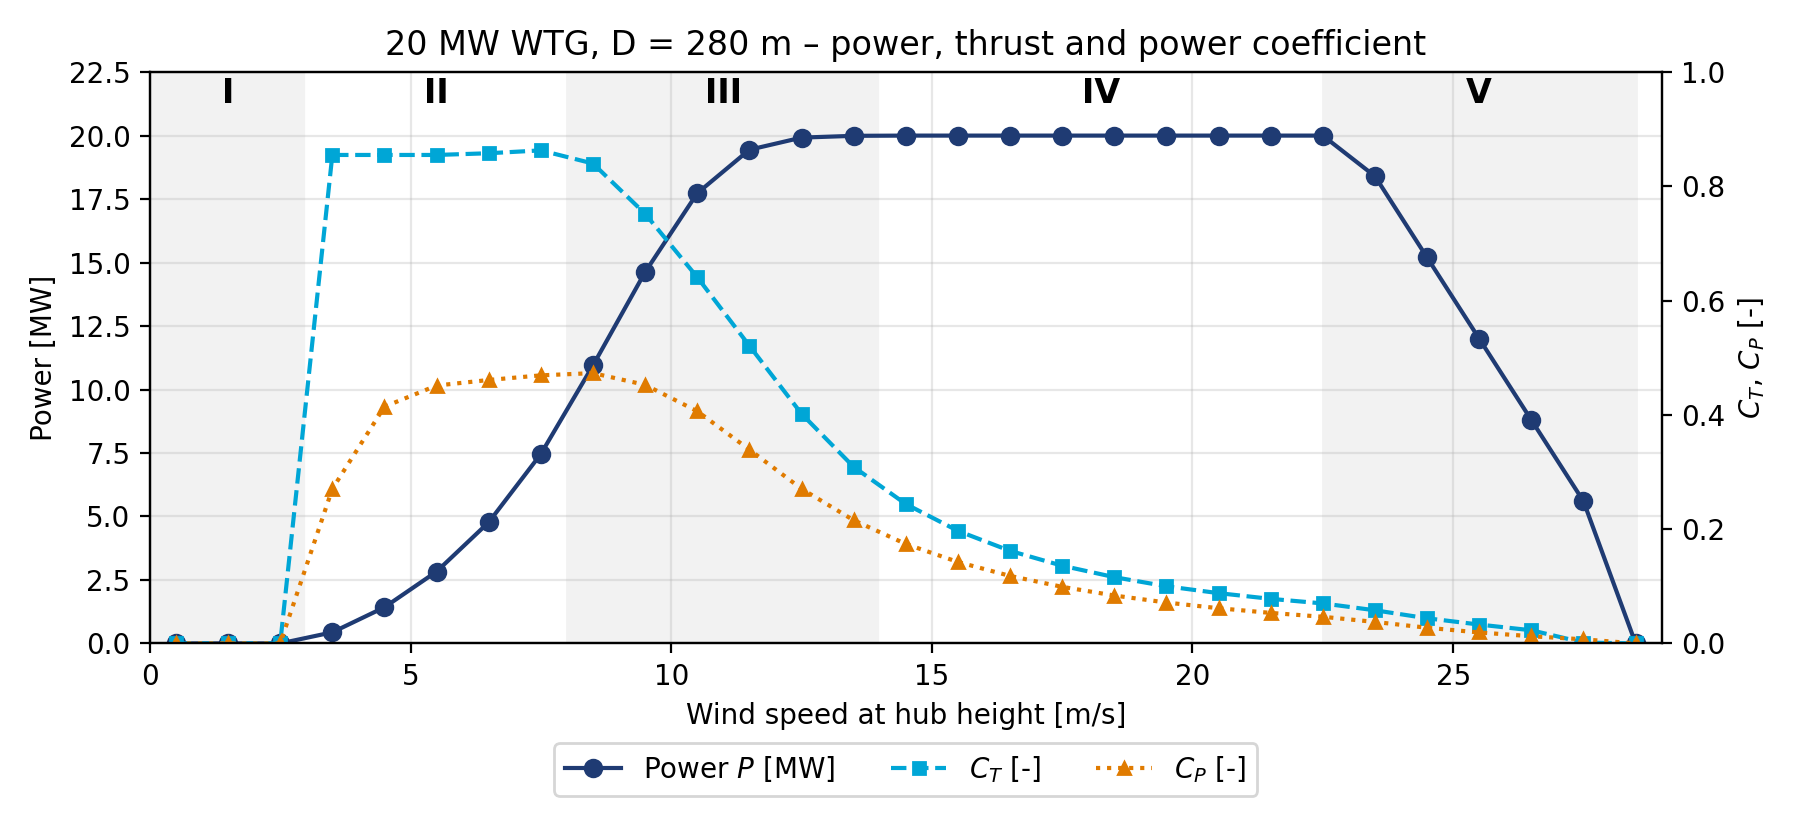
\includegraphics[width=0.85\textwidth]
    {figures/electrical/p1_power_thrust_areas.png}
    \caption{Power curve, thrust coefficient and power coefficient of the $20\,\mathrm{MW}$ WTG with operational areas I--V.}
    \label{fig:elec-curves}
\end{figure}

\begin{table}[H]
    \centering
    \caption{Operational areas, time share and share of the single-WTG energy yield.}
    \label{tab:elec-areas}
    \begin{tabular}{lcccc}
        \hline
        Area & Wind speed & Time & Hours & Energy \\
        & [m/s] & [\%] & [h/yr] & [\%] \\
        \hline
        I   & $< 3$       & 5.7  & 503   & 0.0  \\
        II  & 3 -- 8      & 37.1 & 3249  & 12.9 \\
        III & 8 -- 14     & 44.4 & 3892  & 64.7 \\
        IV  & 14 -- 22.5  & 12.1 & 1057  & 21.4 \\
        V   & 22.5 -- 28  & 0.7  & 63    & 1.1  \\
        \hline
    \end{tabular}
\end{table}

\subsection{Challenge of Operational Area I}
\label{sec:elec-area1}
\begin{quote}
\emph{What is the challenge of operational area I for the power balance in power systems? [1 pts]}
\end{quote}

In area I the wind speed is below cut-in, and the WTG produces no power at all. The grid still has to keep generation equal to load plus losses at every moment, so the whole load must then be covered by other sources: dispatchable plants, storage, demand response or imports. Low wind usually affects a whole region at once, so long calm periods hit all wind parks in that region together and do not average out. At this site area I occurs $5.7\,\%$ of the year (about $500\,\mathrm{h}$, Table~\ref{tab:elec-areas}). The challenge is that wind power adds almost no firm capacity. The system must keep nearly all of its conventional backup capacity available, even though that capacity runs only a few hours a year. Each time the wind crosses the cut-in speed, the park also switches between zero and some output, and the other units must follow these steps.

\subsection{Challenges of Operational Area III}
\label{sec:elec-area3}
\begin{quote}
\emph{What are two challenges of operational area III for keeping the power balance? [2 pts]}
\end{quote}

Area III (variable pitch, about $8$--$14\,\mathrm{m/s}$) is the steepest part of the power curve (Figure~\ref{fig:elec-dpdv}). It is also where the turbine runs most often ($44\,\%$ of the time) and where it produces most of its energy ($65\,\%$). This creates two challenges:

\begin{enumerate}
    \item \textbf{Large and fast power variations.} One WTG changes its output by up to $3.7\,\mathrm{MW}$ per $\mathrm{m/s}$ ($18\,\%$ of rated per $\mathrm{m/s}$). For the 80-WTG park, including wakes, this reaches about $255\,\mathrm{MW}$ per $\mathrm{m/s}$, or $16\,\%$ of installed capacity. Normal turbulence and passing weather fronts therefore cause large ramps. The system operator must balance these with fast reserves and the ramping ability of other units.
    \item \textbf{Amplified forecast errors.} Power is planned day-ahead and intraday from wind speed forecasts. In area III a forecast error of only $1\,\mathrm{m/s}$ becomes a power error of hundreds of MW for one park. The resulting imbalances must be covered by reserve capacity and cost balancing energy. In addition, the WTG runs at its maximum available power, so it can only regulate downwards. It cannot help to close a shortage unless it is curtailed beforehand.
\end{enumerate}

\begin{figure}[H]
    \centering
    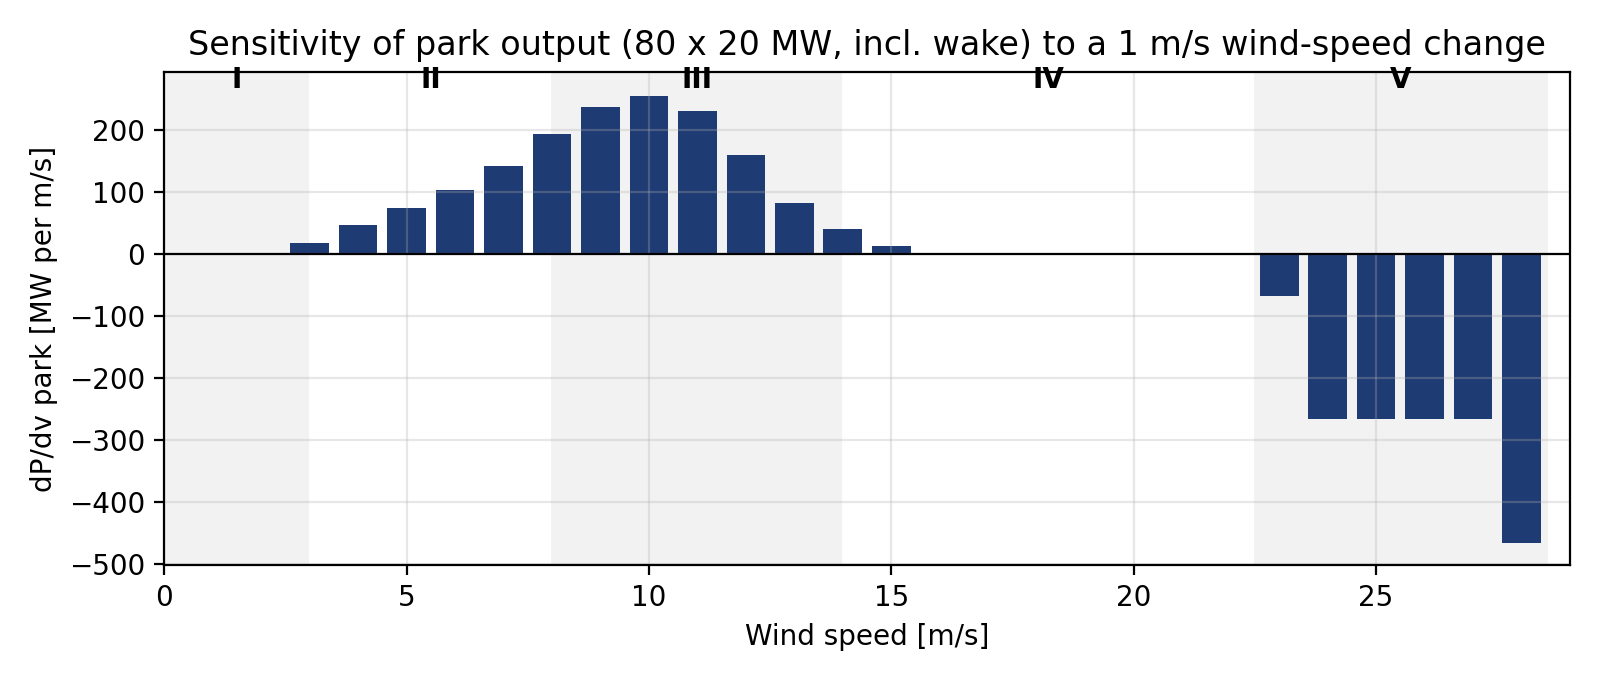
\includegraphics[width=0.8\textwidth]
    {figures/electrical/p1_sensitivity_dPdv.png}
    \caption{Change of park output for a $1\,\mathrm{m/s}$ change of wind speed (80 WTGs including wake).}
    \label{fig:elec-dpdv}
\end{figure}

\subsection{Area V versus a Hard Cut-Out}
\label{sec:elec-area5}
\begin{quote}
\emph{Older wind turbine types had a `hard cut-out' at a specific wind speed. The wind turbine would stop producing power when the wind speed would reach 25 m/s. It would start producing power again when the wind speed would have dropped at around 22 m/s. What are two benefits for power system operation of area V compared to a `hard cut-out' at a specific high wind speed, as is the case for older wind turbines? [2 pts]}
\end{quote}

To illustrate the difference, a synthetic storm passing over the 80-WTG park was simulated (Figure~\ref{fig:elec-storm}). The turbines see slightly different wind speeds, and each control strategy was applied to every turbine. Two benefits follow:

\begin{enumerate}
    \item \textbf{No sudden loss of a large block of generation.} With a hard cut-out, all WTGs in a park (and in neighbouring parks) stop within minutes once the storm passes $25\,\mathrm{m/s}$. For the system this is like the trip of a large power plant: frequency drops, and large, fast and expensive reserves are needed. In area V the output ramps down linearly between $22.5$ and $28\,\mathrm{m/s}$, so the park output falls gradually. In the simulation the largest 10-minute drop falls from about $700\,\mathrm{MW}$ (hard cut-out) to about $290\,\mathrm{MW}$ (area V) for the $1.6\,\mathrm{GW}$ park.
    \item \textbf{No hysteresis, so faster and more predictable recovery.} After a hard cut-out the WTG restarts only below $22\,\mathrm{m/s}$, so it stays off for hours while the wind would already allow production. Output then returns in large steps. In area V the turbine stays connected and follows the wind continuously. Its output is easier to forecast, it keeps supplying grid services such as reactive power and voltage control, and it avoids start/stop cycles. In the simulated storm the park produces about $15\,\%$ more energy ($48.4$ against $42.1\,\mathrm{GWh}$).
\end{enumerate}

\begin{figure}[H]
    \centering
    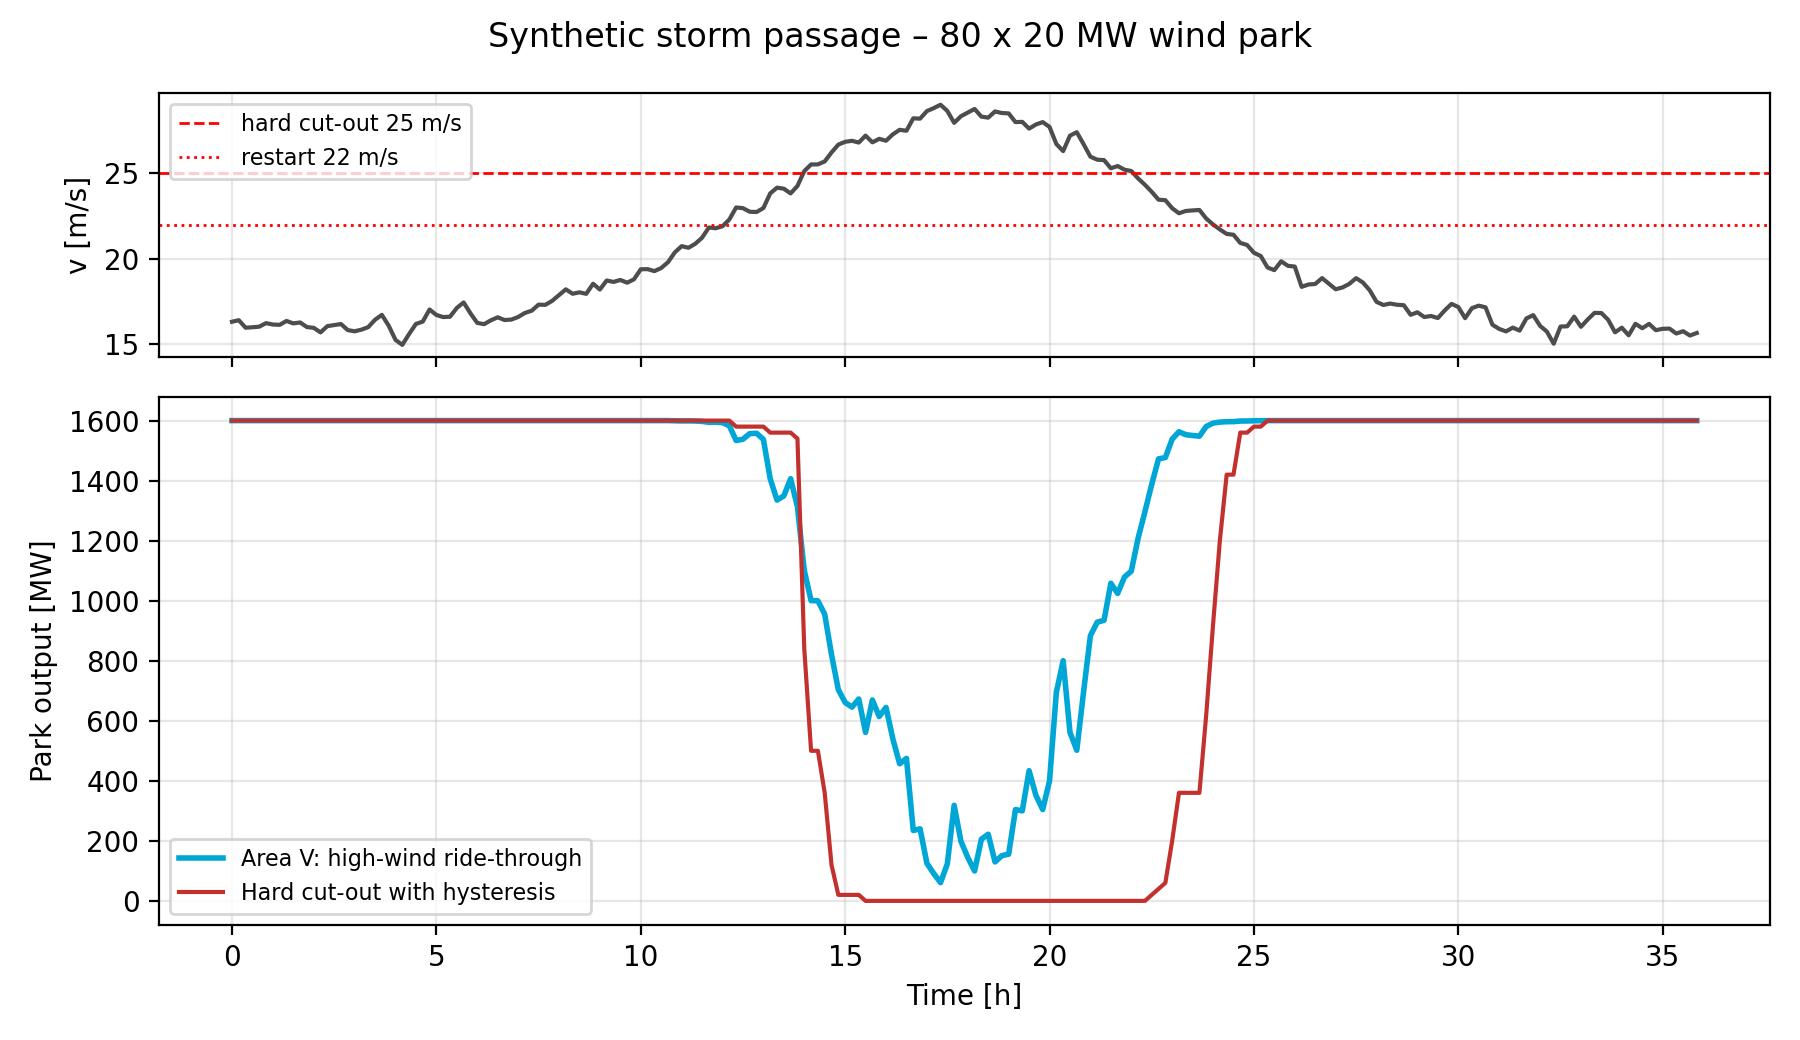
\includegraphics[width=0.85\textwidth]
    {figures/electrical/p1_storm_hwrt_vs_hardcutout.png}
    \caption{Synthetic storm passage: park output with high-wind ride-through (area V) and with a hard cut-out at $25\,\mathrm{m/s}$ and restart at $22\,\mathrm{m/s}$.}
    \label{fig:elec-storm}
\end{figure}

\subsection{Wind Speeds with Negligible Wake Effects}
\label{sec:elec-wake-negl}
\begin{quote}
\emph{Offshore wind parks consist of a cluster of wind turbines. The power production by such a cluster of wind turbines is dependent on the wake effects: the power production of wind turbines may be reduced in the wake of other turbines. In the Excel file, tab `WTG Yield Wake', an omni-directional wake effect for a wind park of 80 WTGs is provided for wind speeds at hub height. For this wind park, at what wind speeds are the wake effects negligible? [1 pts]}
\end{quote}

The wake effects are negligible between about $14.5$ and $22.5\,\mathrm{m/s}$, which is the rated-power range (area IV). The park efficiency is $99.2\,\%$ at $14.5\,\mathrm{m/s}$ and $99.94\,\%$ from $15.5$ to $22.5\,\mathrm{m/s}$, a loss of only $0.06\,\%$ (Figure~\ref{fig:elec-eta}). Above $22.5\,\mathrm{m/s}$ the wake even increases production (Section~\ref{sec:elec-wake-high}). Below $14\,\mathrm{m/s}$ the losses are significant.

\begin{figure}[H]
    \centering
    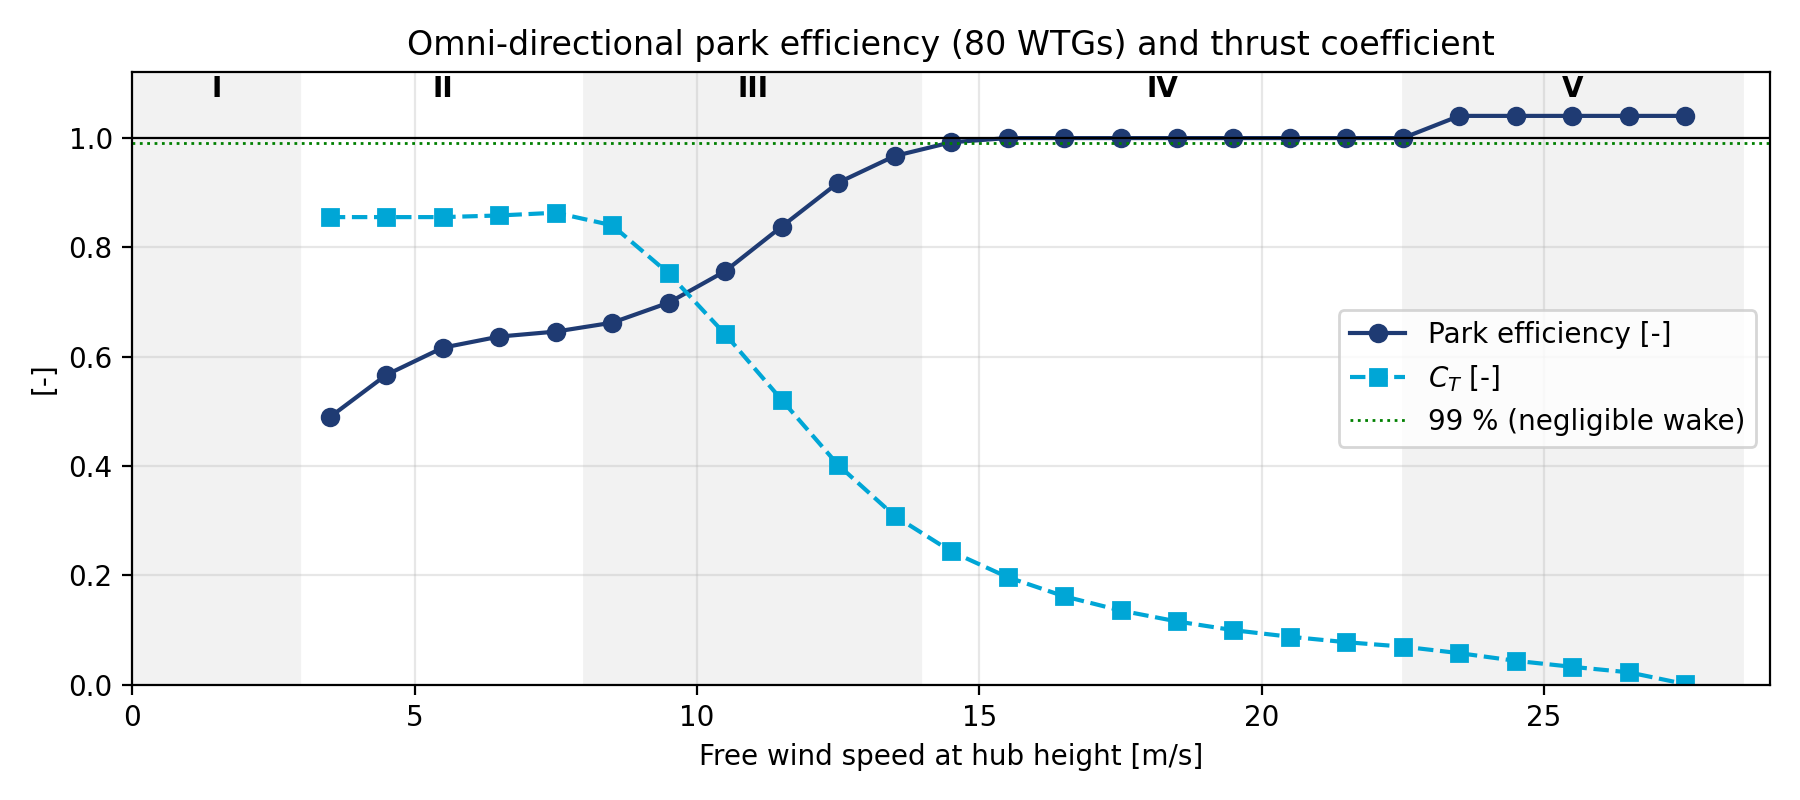
\includegraphics[width=0.85\textwidth]
    {figures/electrical/p1_park_efficiency_ct.png}
    \caption{Omni-directional park efficiency of the 80-WTG park and thrust coefficient versus free wind speed.}
    \label{fig:elec-eta}
\end{figure}

\subsection{Wake Impact in Areas II, III and IV}
\label{sec:elec-wake-areas}
\begin{quote}
\emph{Explain for operational areas II, III and IV what impact the wake effects have on power production of an offshore wind park. Consider the thrust curve as part of your answer. [2 pts]}
\end{quote}

The velocity deficit in a wake grows with the thrust coefficient. Just behind the rotor, momentum theory gives

\begin{equation}
    \frac{u_{wake}}{u_\infty} \approx \sqrt{1 - C_T},
    \label{eq:elec-wake}
\end{equation}

so a WTG that takes more momentum out of the flow leaves a slower wake. Table~\ref{tab:elec-wakeareas} quantifies the impact per area.

\begin{itemize}
    \item \textbf{Area II} ($3$--$8\,\mathrm{m/s}$): $C_T$ is high and nearly constant ($\approx 0.86$), so the wake deficit is largest. Power scales with $v^3$, so a waked WTG loses a large share of its output. The park efficiency is only $49$--$65\,\%$. The power levels are low, so the absolute loss ($375\,\mathrm{GWh/yr}$) is about $27\,\%$ of the total wake loss.
    \item \textbf{Area III} ($8$--$14\,\mathrm{m/s}$): the blades pitch and $C_T$ falls from $0.84$ to about $0.3$. The wake deficit therefore decreases, and the park efficiency rises from $66\,\%$ to $97\,\%$. However, this area holds most of the energy and the power curve is steepest here, so even a small deficit costs a lot of power. Area III causes about $73\,\%$ of the wake losses ($1025\,\mathrm{GWh/yr}$). In effect, the wakes shift the park power curve to higher wind speeds, so the park reaches rated power later than a single WTG.
    \item \textbf{Area IV} ($14$--$22.5\,\mathrm{m/s}$): $C_T$ is low ($<0.25$), so the wakes are weak. Even a waked WTG still sees a wind speed above rated and keeps producing $20\,\mathrm{MW}$. The wake loss is negligible ($4.6\,\mathrm{GWh/yr}$).
\end{itemize}

\begin{table}[H]
    \centering
    \caption{Annual gross and net (including wake) park production per operational area.}
    \label{tab:elec-wakeareas}
    \begin{tabular}{lcccc}
        \hline
        Area & Gross & Net & Wake loss & Share of wake loss \\
        & [GWh/yr] & [GWh/yr] & [GWh/yr] & [\%] \\
        \hline
        II  & 1017.0 & 642.3  & 374.8  & 26.7 \\
        III & 5111.0 & 4086.2 & 1024.8 & 73.1 \\
        IV  & 1691.5 & 1686.9 & 4.6    & 0.3  \\
        V   & 85.7   & 87.4   & $-1.8$ & $-0.1$ \\
        \hline
        Total & 7905.2 & 6502.8 & 1402.4 & 100 \\
        \hline
    \end{tabular}
\end{table}

\subsection{Wake Benefit at Very High Wind Speeds}
\label{sec:elec-wake-high}
\begin{quote}
\emph{At high wind speeds (23.5 -- 27.5 m/s), the wake effect slightly increases power production of the wind park as a whole, compared to an individual wind turbine. Provide a technical explanation for this effect of wind park wakes. In your answer, consider that wake involves a lower wind speed behind a wind turbine and consider the power curve of the turbine at that wind speed range. [1 pts]}
\end{quote}

Between $22.5$ and $28\,\mathrm{m/s}$ (area V) the power curve has a negative slope of about $-3.2\,\mathrm{MW}$ per $\mathrm{m/s}$: the WTG reduces its output as the wind speed rises, to limit loads. A WTG in the wake of another turbine sees a lower wind speed than the free stream, so it operates higher on this descending part of the curve and produces more. For example, a free-stream WTG at $24.5\,\mathrm{m/s}$ produces $15.2\,\mathrm{MW}$, while a waked WTG that sees $23.5\,\mathrm{m/s}$ produces $18.4\,\mathrm{MW}$. Some downstream turbines may even stay below $22.5\,\mathrm{m/s}$ and produce rated power. $C_T$ is very small at these wind speeds ($<0.06$), so the deficits are small and the net gain is limited to about $4\,\%$ (park efficiency $1.04$).

\subsection{Opportunities of a Larger Rotor for the Owner}
\label{sec:elec-rotor-owner}
\begin{quote}
\emph{In the past decade, wind turbines have become much larger. This is true for the generator sizes [MW], but even more for the rotor diameters [m] which have become larger also relative to generator size. Compare two identical wind turbines with a fixed capacity [MW] but with different rotor sizes. Discuss two opportunities of a larger wind turbine rotor for the owner of a wind park. Include the operational areas of relevance in your answer. [2 pts]}
\end{quote}

To quantify the effect, the same $20\,\mathrm{MW}$ generator was combined with a $236\,\mathrm{m}$ rotor ($457\,\mathrm{W/m^2}$) and a $280\,\mathrm{m}$ rotor ($325\,\mathrm{W/m^2}$). Both use the same aerodynamic $C_P$ curve, the same high-wind control and the same wind distribution (Figure~\ref{fig:elec-rotor}, Table~\ref{tab:elec-rotor}). The model is simplified: it uses $C_{P,max}=0.47$ up to rated power, so the absolute yields differ slightly from the template.

\begin{enumerate}
    \item \textbf{More energy and a higher capacity factor (areas II and III).} The captured power scales with the swept area, $P \propto D^2 v^3$. The larger rotor therefore produces more at every wind speed below rated and reaches rated power at a lower wind speed ($10.5$ instead of $12.5\,\mathrm{m/s}$). Area III shifts to lower wind speeds and area IV becomes wider. The annual yield rises by about $16\,\%$ (capacity factor $49.8\,\% \rightarrow 57.9\,\%$), and the hours at rated power rise from about $2000$ to $3300\,\mathrm{h/yr}$.
    \item \textbf{Better use of the expensive electrical system and higher revenue per MWh.} The generator, converter, inter-array cables, substation and export cables are sized on MW, not on rotor size. A larger rotor sends more MWh through the same electrical infrastructure, which lowers the levelised cost of energy and the grid connection cost per MWh. Most of the extra energy is produced at low to moderate wind speeds (areas II and III). In those hours total wind production in the market is lower, so electricity prices are usually higher and the market value per MWh improves.
\end{enumerate}

The trade-offs are higher rotor loads, larger foundations and stronger wakes, which require a larger turbine spacing.

\begin{figure}[H]
    \centering
    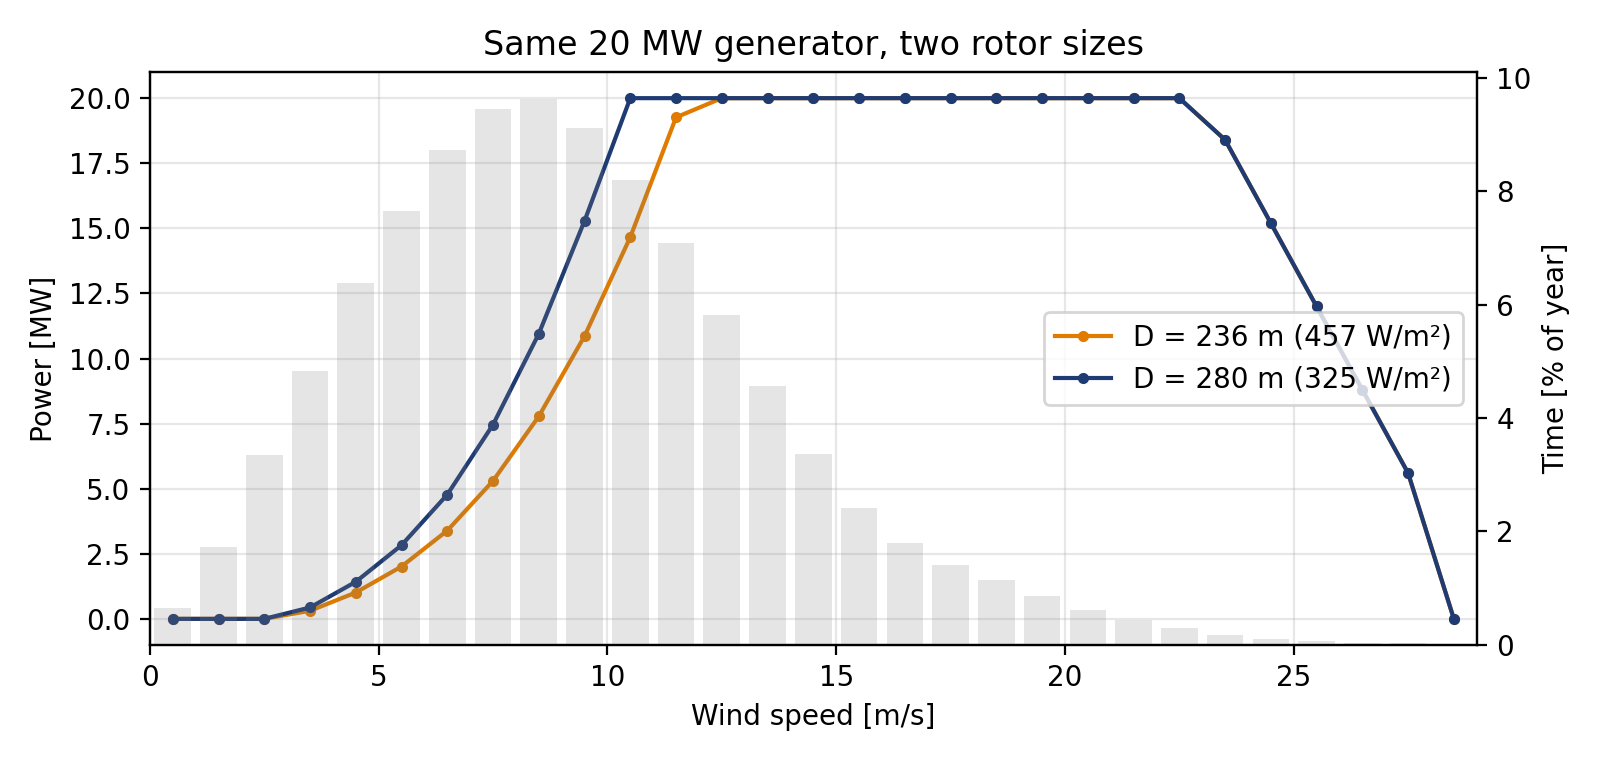
\includegraphics[width=0.75\textwidth]
    {figures/electrical/p1_rotor_size_comparison.png}
    \caption{Power curves of a $20\,\mathrm{MW}$ WTG with a $236\,\mathrm{m}$ and a $280\,\mathrm{m}$ rotor, with the wind speed distribution of the template.}
    \label{fig:elec-rotor}
\end{figure}

\begin{table}[H]
    \centering
    \caption{Comparison of two rotor sizes for the same $20\,\mathrm{MW}$ generator (simplified model).}
    \label{tab:elec-rotor}
    \begin{tabular}{lcc}
        \hline
        Quantity & $D=236\,\mathrm{m}$ & $D=280\,\mathrm{m}$ \\
        \hline
        Specific rating [$\mathrm{W/m^2}$] & 457 & 325 \\
        Rated power reached at [m/s] & 12.5 & 10.5 \\
        Annual energy yield [MWh/yr] & 87,179 & 101,366 \\
        Capacity factor [\%] & 49.8 & 57.9 \\
        Hours at rated power [h/yr] & 1993 & 3332 \\
        Maximum $dP/dv$ [MW per m/s] & 4.60 & 4.71 \\
        Mean $|\Delta P|$ for a $1\,\mathrm{m/s}$ forecast error [MW] & 1.68 & 1.74 \\
        \quad relative to mean output [\%] & 16.9 & 15.0 \\
        Standard deviation / mean of output [-] & 0.76 & 0.67 \\
        \hline
    \end{tabular}
\end{table}

\subsection{A Larger Rotor from a Power System Perspective}
\label{sec:elec-rotor-system}
\begin{quote}
\emph{Argue if a larger rotor could be beneficial from a power system operation point of view. Consider variations of the power produced and wind forecast errors in your answer. [2 pts]}
\end{quote}

On balance, a larger rotor (lower specific rating) benefits power system operation.

Regarding variations of the power produced, the WTG reaches rated power at a lower wind speed, so it spends far more time in area IV ($67\,\%$ more hours at rated). In area IV, wind fluctuations do not change the output at all. Output in low winds is also higher, so there are fewer hours near zero. The production profile becomes flatter and more like baseload: relative variability (standard deviation divided by mean) drops from $0.76$ to $0.67$, and the capacity factor rises, so the grid connection is used better. One drawback is that the steep part of the curve (area III) moves to $7$--$10\,\mathrm{m/s}$, the most frequent wind speeds, so ramps occur in more common weather conditions.

Regarding wind forecast errors, a forecast error has no effect on power in area IV, and the larger rotor widens this area. More hours of the year are therefore insensitive to forecast errors. In absolute terms the expected power error for a $1\,\mathrm{m/s}$ forecast error is almost unchanged ($1.68$ against $1.74\,\mathrm{MW}$). Relative to the higher mean output it is lower ($16.9\,\% \rightarrow 15.0\,\%$), so each MWh delivered needs less balancing reserve.

A larger rotor therefore gives a smoother, more predictable and firmer supply per MW of grid capacity. The main side effect is more hours with high wind output at moderate wind speeds. In systems with a very high wind share, this can increase curtailment or the number of hours with low or negative prices.

\section{Inter-Array Cabling Losses}
\label{sec:elec-part2}

\subsection{Cable Data}
\label{sec:elec-cable-data}
The three inter-array cable (IAC) types of the assignment are listed in Table~\ref{tab:elec-cables}. The WTGs are $20\,\mathrm{MW}$ units operating at $\cos\varphi = 0.95$. Wake losses are neglected, which gives a conservative (high) estimate of the cable currents.

\begin{table}[H]
    \centering
    \caption{Inter-array cable types at $66\,\mathrm{kV}$ and resulting maximum number of $20\,\mathrm{MW}$ WTGs.}
    \label{tab:elec-cables}
    \begin{tabular}{lcccccc}
        \hline
        Cable & Type & Ampacity & $R$ & Ampacity$/I_{WTG}$ & $n_{max}$ & Loading at $n_{max}$ \\
        & [$\mathrm{mm^2}$] & [A] & [$\Omega$/km] & [-] & [-] & [\%] \\
        \hline
        Cable 1 & 400 & 424 & 0.101 & 2.30 & 2 & 86.9 \\
        Cable 2 & 630 & 584 & 0.063 & 3.17 & 3 & 94.6 \\
        Cable 3 & 800 & 750 & 0.037 & 4.07 & 4 & 98.2 \\
        \hline
    \end{tabular}
\end{table}

\subsection{Rated Current per Wind Turbine}
\label{sec:elec-current}
\begin{quote}
\emph{The type indicates the cross-section of the aluminium conductor [mm$^2$]. The ampacity is the maximum current [A] the cable type is designed to handle. Assume you are using 20 MW offshore wind turbines. For the calculation, assume that every wind turbine operates at cos $\varphi$ = 0.95 and do not consider any wake losses (conservative estimate for the current in the cables). Calculate the rated current per wind turbine. [2 pts]}
\end{quote}

The apparent power of one WTG is

\begin{equation}
    S_{WTG} = \frac{P}{\cos\varphi} = \frac{20\,\mathrm{MW}}{0.95} = 21.05\,\mathrm{MVA}.
    \label{eq:elec-swtg}
\end{equation}

With the three-phase relation $S = \sqrt{3}\,U_{ph-ph}\,I$, the rated current at $66\,\mathrm{kV}$ is

\begin{equation}
    I_{WTG} = \frac{S_{WTG}}{\sqrt{3}\,U} = \frac{21.05\times10^{6}\,\mathrm{VA}}{\sqrt{3}\cdot 66\times10^{3}\,\mathrm{V}} = 184.2\,\mathrm{A}.
    \label{eq:elec-iwtg}
\end{equation}

The template rounds the WTG rating to $21.1\,\mathrm{MVA}$, which gives $184.6\,\mathrm{A}$. That value is used in the `IAC' tab.

\subsection{Maximum Number of WTGs per Cable Type}
\label{sec:elec-nmax}
\begin{quote}
\emph{Determine the maximum number of wind turbines that can be connected to Cable 1, Cable 2 and Cable 3 without exceeding the ampacity. [2 pts]}
\end{quote}

The maximum number of WTGs per cable is

\begin{equation}
    n_{max} = \left\lfloor \frac{I_{ampacity}}{I_{WTG}} \right\rfloor,
    \label{eq:elec-nmax}
\end{equation}

which gives $424/184.2 = 2.30$, so \textbf{2 WTGs} on Cable 1 ($368\,\mathrm{A}$); $584/184.2 = 3.17$, so \textbf{3 WTGs} on Cable 2 ($552\,\mathrm{A}$); and $750/184.2 = 4.07$, so \textbf{4 WTGs} on Cable 3 ($737\,\mathrm{A}$), as summarised in Table~\ref{tab:elec-cables}.

\subsection{Annual IAC Losses of the String}
\label{sec:elec-iac-losses}
\begin{quote}
\emph{Assume that you want to use the cheapest cable type where possible. Review the Excel file, tab `IAC' and, using your answers above, complete all yellow cells. What is the annual electricity loss as a percentage of the yield of the WTGs on the string? [2 pts]}
\end{quote}

The string in the `IAC' tab connects four WTGs. Each cable section is named after the WTG at its upstream end and carries the power of all WTGs before it. For each section, the cheapest (smallest) cable whose ampacity is not exceeded was selected. Table~\ref{tab:elec-yellow} shows the completed yellow cells.

\begin{table}[H]
    \centering
    \caption{Completed yellow cells of the `IAC' tab (rows 11--13).}
    \label{tab:elec-yellow}
    \begin{tabular}{lcccc}
        \hline
        Section & WTG 1 & WTG 2 & WTG 3 & WTG 4 \\
        \hline
        Number of WTGs on IAC section & 1 & 2 & 3 & 4 \\
        Section length [km] & 2.5 & 2.5 & 2.0 & 1.5 \\
        Nominal current [A] (E11:H11) & 184.6 & 369.2 & 553.7 & 738.3 \\
        IAC cable (E12:H12) & 1 & 1 & 2 & 3 \\
        Resistance [$\Omega$/km] (E13:H13) & 0.101 & 0.101 & 0.063 & 0.037 \\
        Loading [\%] & 43.5 & 87.1 & 94.8 & 98.4 \\
        \hline
    \end{tabular}
\end{table}

Column D (rows 18--46) holds the apparent power per wind speed bin, $S(v) = P(v)/0.95$. The loss in section $k$ follows the template formula, in which the current scales with the actual output:

\begin{equation}
    P_{loss,k}(v) = 3\left(\frac{S(v)}{S_{nom}}\,I_{nom,k}\right)^2 R_k L_k.
    \label{eq:elec-ploss}
\end{equation}

Multiplying by the hours in each bin and summing over all bins and sections gives the annual string losses (cell K48) of $1341.6\,\mathrm{MWh/yr}$. The energy yield of the four WTGs (cell K49) is

\begin{equation}
    E_{string} = 4\sum_{v} P(v)\,h(v) = 394{,}990\,\mathrm{MWh/yr},
    \label{eq:elec-yield}
\end{equation}

so the annual loss (cell K50) is

\begin{equation}
    \frac{E_{loss}}{E_{string}} = \frac{1341.6}{394{,}990} = 0.34\,\%.
    \label{eq:elec-losspct}
\end{equation}

The annual IAC loss is therefore \textbf{0.34\,\% of the WTG yield}. At full power the instantaneous loss is $334\,\mathrm{kW}$ ($0.42\,\%$ of $80\,\mathrm{MW}$). The annual percentage is lower because losses scale with $I^2$ and the WTGs run below rated most of the time. Sections 3 and 4, which carry the highest currents, cause the largest losses (Figure~\ref{fig:elec-iac}).

\begin{figure}[H]
    \centering
    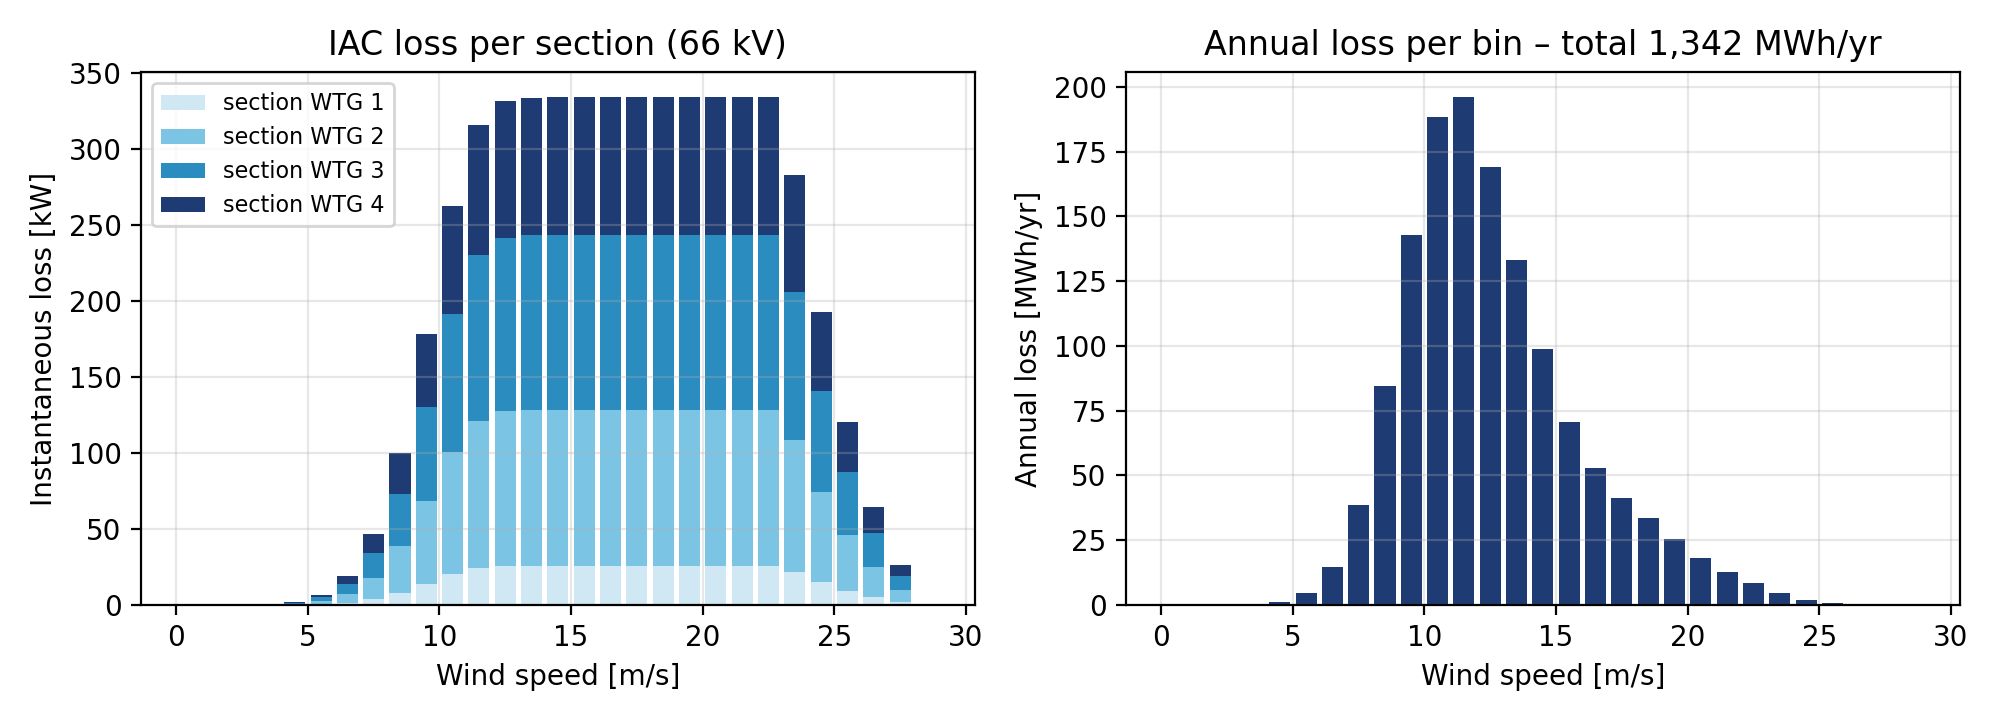
\includegraphics[width=\textwidth]
    {figures/electrical/p2_iac_losses.png}
    \caption{Left: instantaneous IAC losses per string section versus wind speed at $66\,\mathrm{kV}$. Right: annual losses per wind speed bin.}
    \label{fig:elec-iac}
\end{figure}

\subsection{Number of WTGs on Cable 1 at 132 kV}
\label{sec:elec-132-n}
\begin{quote}
\emph{Assume that the voltage level of the cables would be 132 kV instead of 66 kV and that the conductor resistance would be the same. How many WTGs of 20 MW could be connected to Cable 1 if it would be at 132 kV? [1 pt]}
\end{quote}

Doubling the voltage halves the current per WTG:

\begin{equation}
    I_{WTG,132} = \frac{21.05\,\mathrm{MVA}}{\sqrt{3}\cdot 132\,\mathrm{kV}} = 92.1\,\mathrm{A},
    \qquad \frac{424}{92.1} = 4.60.
    \label{eq:elec-i132}
\end{equation}

At $132\,\mathrm{kV}$, Cable 1 can therefore connect \textbf{4 WTGs} ($80\,\mathrm{MW}$, $368\,\mathrm{A}$), twice as many as at $66\,\mathrm{kV}$.

\subsection{Loss Reduction at 132 kV}
\label{sec:elec-132-loss}
\begin{quote}
\emph{How much would the annual losses on the wind turbine string be reduced if the voltage level would be increased to 132 kV, everything else being equal? Explain your answer. [1 pt]}
\end{quote}

The power is the same, so $S = \sqrt{3}UI$ gives half the current at twice the voltage. Ohmic losses scale with the square of the current, $P_{loss} = 3I^2R$. With the same cables (same $R$ and $L$),

\begin{equation}
    \frac{P_{loss,132}}{P_{loss,66}} = \left(\frac{66}{132}\right)^2 = \frac{1}{4}.
    \label{eq:elec-lossratio}
\end{equation}

The annual losses drop by \textbf{75\,\%}, from $1341.6\,\mathrm{MWh/yr}$ ($0.34\,\%$) to $335.4\,\mathrm{MWh/yr}$ ($0.085\,\%$), a saving of about $1006\,\mathrm{MWh/yr}$ per string. This is why array systems have moved from $33$ to $66\,\mathrm{kV}$ and now to $132\,\mathrm{kV}$: a higher voltage means a lower current and lower losses. At $132\,\mathrm{kV}$ the cheaper Cable 1 could also be used for the whole string. The losses would then be $562\,\mathrm{MWh/yr}$, still $58\,\%$ lower than the $66\,\mathrm{kV}$ base case, at a lower cable cost. In return, the higher voltage requires more expensive switchgear and WTG transformers with a higher insulation level.

\section{Offshore Wind Park Electrical Design}
\label{sec:elec-part3}

\subsection{Single-Line Diagram}
\label{sec:elec-sld}
The single-line diagram (Figure~\ref{fig:elec-sld}) shows 12 strings in six pairs. Each pair connects 11 WTGs of $12\,\mathrm{MVA}$ ($132\,\mathrm{MVA}$) to one $66\,\mathrm{kV}$ busbar section, which feeds one secondary winding of a $220/66/66\,\mathrm{kV}$ transformer. The installed wind power is $66 \times 12\,\mathrm{MVA} = 792\,\mathrm{MVA}$. The substation has three transformers rated $264/132/132\,\mathrm{MVA}$ (ONAN) and $400/200/200\,\mathrm{MVA}$ (ONAF), and three $220\,\mathrm{kV}$ export cables, one per transformer bay. Both the $66\,\mathrm{kV}$ and the $220\,\mathrm{kV}$ busbars have bus-section couplers.

\begin{figure}[H]
    \centering
    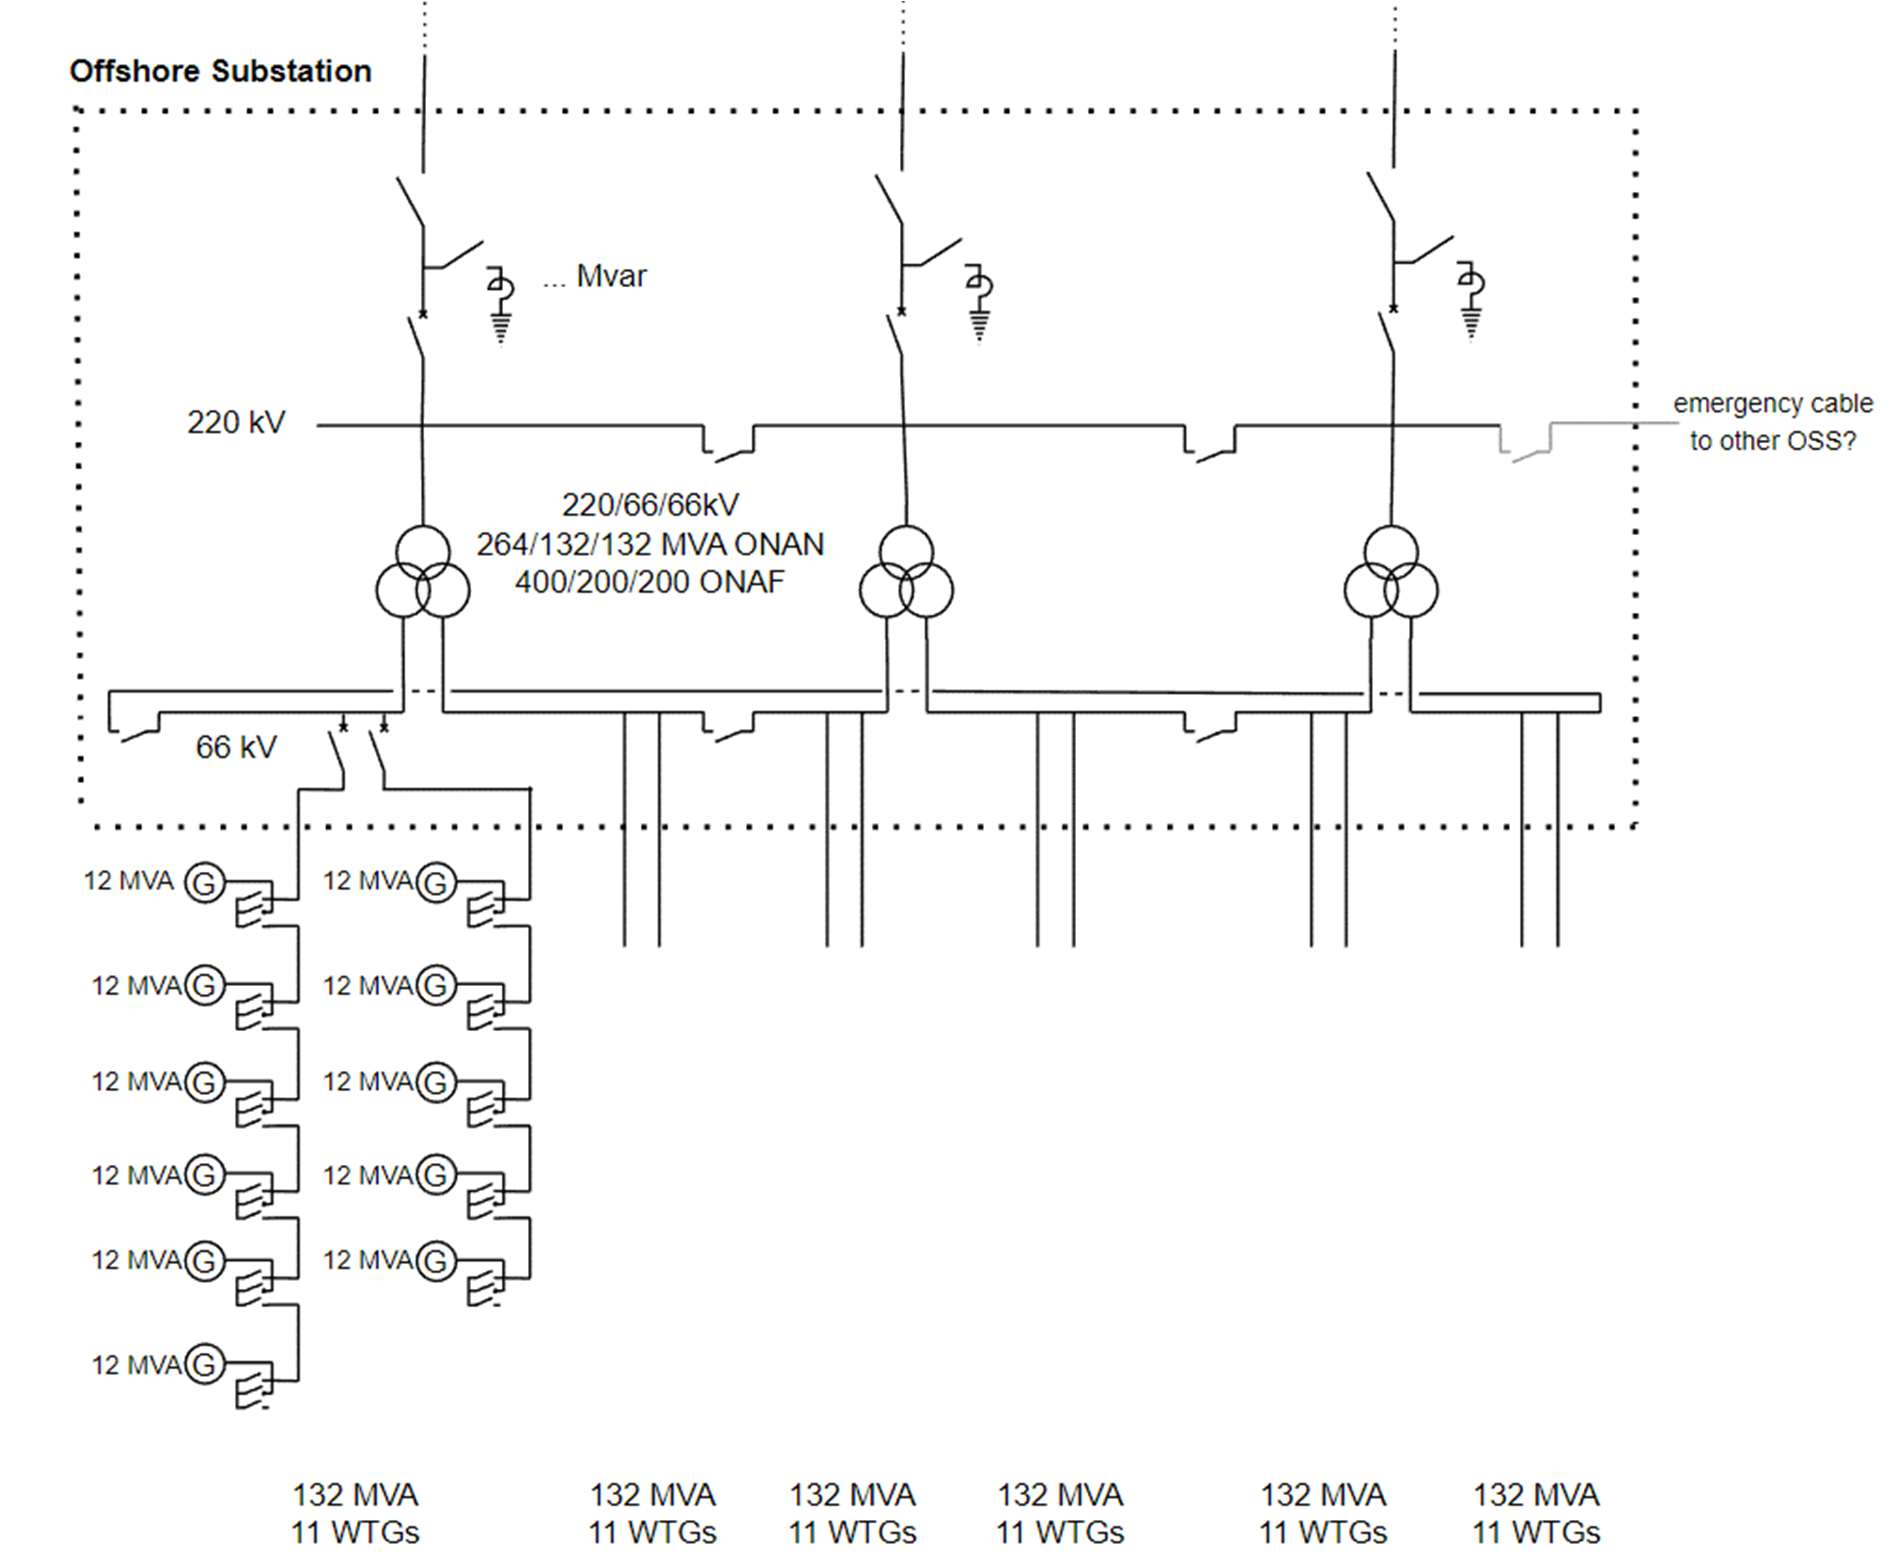
\includegraphics[width=0.85\textwidth]
    {figures/electrical/given_single_line_diagram.png}
    \caption{Single-line diagram of the offshore substation, as given in the assignment (only two of the twelve strings are drawn).}
    \label{fig:elec-sld}
\end{figure}

\subsection{Power over One Export Cable}
\label{sec:elec-export-power}
\begin{quote}
\emph{For normal operation, how much power would flow over one export cable? [1 pts]}
\end{quote}

In normal operation the three transformers and three export cables share the park output equally:

\begin{equation}
    S_{cable} = \frac{66 \times 12\,\mathrm{MVA}}{3} = \frac{792\,\mathrm{MVA}}{3} = 264\,\mathrm{MVA}.
    \label{eq:elec-scable}
\end{equation}

Each export cable therefore carries \textbf{264\,MVA}, equal to the ONAN rating of one transformer. This corresponds to a current of $264\,\mathrm{MVA}/(\sqrt{3}\cdot 220\,\mathrm{kV}) = 693\,\mathrm{A}$. Collection-system losses and reactive power are neglected.

\subsection{Transformer Winding Currents}
\label{sec:elec-winding}
\begin{quote}
\emph{For normal operation, how much current is flowing on one 66 kV winding of the transformer? How much current is flowing on the 220 kV winding of the transformer? [2 pts]}
\end{quote}

Each $66\,\mathrm{kV}$ winding is fed by one busbar section with 11 WTGs ($132\,\mathrm{MVA}$), and the $220\,\mathrm{kV}$ winding carries the sum of both secondary windings ($264\,\mathrm{MVA}$):

\begin{equation}
    I_{66} = \frac{132\,\mathrm{MVA}}{\sqrt{3}\cdot 66\,\mathrm{kV}} = 1155\,\mathrm{A},
    \qquad
    I_{220} = \frac{264\,\mathrm{MVA}}{\sqrt{3}\cdot 220\,\mathrm{kV}} = 693\,\mathrm{A}.
    \label{eq:elec-iwinding}
\end{equation}

As a check, $2 \times 1155 / 693 = 3.33 = 220/66$. The current ratio equals the voltage ratio, so power is conserved over the transformer.

\subsection{Redundancy of the Offshore Transformers}
\label{sec:elec-redundancy}
\begin{quote}
\emph{For this exercise, redundancy can be assumed to be the \% of the installed wind power [MVA] over the installed transformer power [MVA]. Assume that there is emergency operation because one of the three transformers has an electrical fault and is out of service (N-1). Assume that all wind turbines are available for power production and the substation has been set so that all wind turbines are connected to the remaining two transformers. What is the level of redundancy [\%] when considering the offshore substation transformers? Support your answer using a short calculation. [2 pts]}
\end{quote}

With one transformer out of service, the two remaining units run at their ONAF (emergency) rating of $400\,\mathrm{MVA}$:

\begin{equation}
    \text{Redundancy} = \frac{S_{wind}}{S_{TR,available}} = \frac{792\,\mathrm{MVA}}{2 \times 400\,\mathrm{MVA}} = \frac{792}{800} = 99\,\%.
    \label{eq:elec-redundancy}
\end{equation}

Each remaining transformer carries $396\,\mathrm{MVA}$ ($1039\,\mathrm{A}$ at $220\,\mathrm{kV}$). Each $66\,\mathrm{kV}$ winding carries $198\,\mathrm{MVA}$ ($1732\,\mathrm{A}$), against its $200\,\mathrm{MVA}$ ONAF rating. The two transformers can therefore export the full park output with $1\,\%$ ($8\,\mathrm{MVA}$) margin, without curtailment, so the transformer design is fully N-1 redundant. Without forced cooling (ONAN) the ratio would be $792/528 = 150\,\%$, and one third of the park would have to be curtailed. Table~\ref{tab:elec-red} compares all cases.

\begin{table}[H]
    \centering
    \caption{Installed wind power versus available transformer capacity.}
    \label{tab:elec-red}
    \begin{tabular}{lcccc}
        \hline
        Case & Transformers & Capacity & Wind/capacity & Margin \\
        & [-] & [MVA] & [\%] & [MVA] \\
        \hline
        Normal, ONAN & 3 & 792  & 100 & 0 \\
        Normal, ONAF & 3 & 1200 & 66  & 408 \\
        N-1, ONAN    & 2 & 528  & 150 & $-264$ \\
        N-1, ONAF    & 2 & 800  & 99  & 8 \\
        \hline
    \end{tabular}
\end{table}

\subsection{Optimal Capacity of the Export Cable Circuits}
\label{sec:elec-export-capacity}
\begin{quote}
\emph{What would be the optimal capacity [MVA] of the export cable circuits? [2 pts]}
\end{quote}

The optimal capacity is about \textbf{264\,MVA per export circuit}, or roughly $700\,\mathrm{A}$ at $220\,\mathrm{kV}$. Three circuits then give $3 \times 264 = 792\,\mathrm{MVA}$, equal to the installed wind power. Three arguments support this choice:

\begin{itemize}
    \item \textbf{A transformer outage does not overload the cables.} The $220\,\mathrm{kV}$ busbar has bus-section couplers. During the N-1 transformer case, the $792\,\mathrm{MVA}$ from the two remaining transformers is spread over all three export cables, so each still carries $264\,\mathrm{MVA}$. A $400\,\mathrm{MVA}$ cable rating, matching the ONAF transformer rating, would only be needed if each cable were tied to its own transformer.
    \item \textbf{Oversizing the cables costs more than it saves.} Export cables are among the most expensive components, and their cost rises with conductor cross-section and installation effort. Sizing every cable for $400\,\mathrm{MVA}$ would only pay off during rare cable outages. If one of three cables is lost, $2 \times 264 = 528\,\mathrm{MVA}$ remains. According to the park duration curve (Figure~\ref{fig:elec-duration}), this still carries the full output $62\,\%$ of the time and $83\,\%$ of the energy during such an outage. The cheap redundancy is in the transformers (fans for ONAF), not in the cables.
    \item \textbf{Undersizing loses energy permanently.} For example, with $3 \times 200\,\mathrm{MVA}$ the park would be curtailed in every high-wind hour and lose about $11\,\%$ of its yield.
\end{itemize}

In practice a small margin above $264\,\mathrm{MVA}$ is chosen. The cable must also carry reactive current: its charging current is only partly compensated by the shunt reactors in the single-line diagram, and the grid code requires reactive power exchange. It must also operate at the lowest allowed voltage. The thermal time constant of the cable allows short overloads.

\begin{figure}[H]
    \centering
    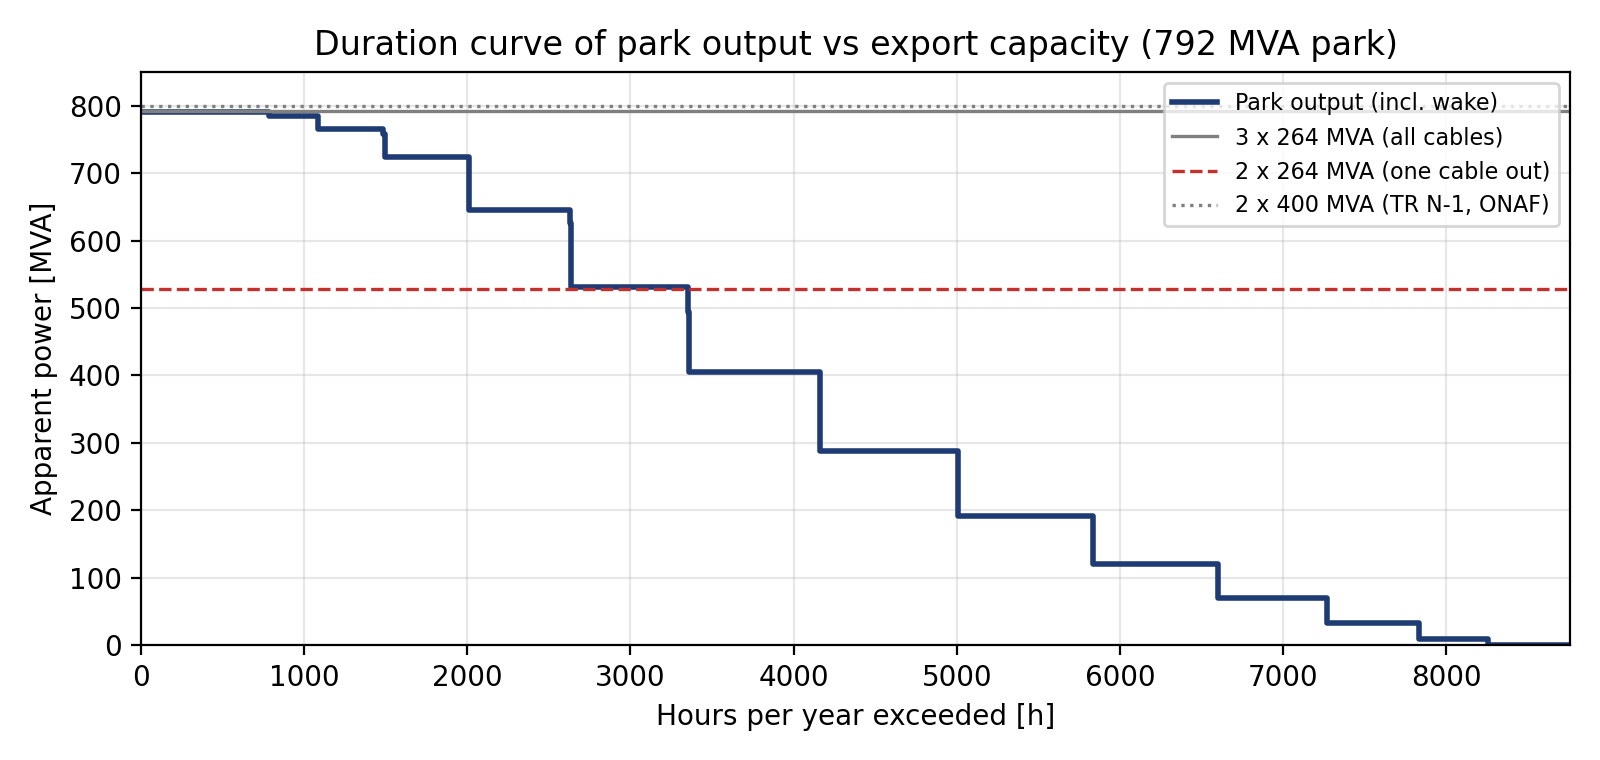
\includegraphics[width=0.75\textwidth]
    {figures/electrical/p3_duration_export_capacity.png}
    \caption{Duration curve of the park output (template wind distribution including wake, scaled to $792\,\mathrm{MVA}$) and export capacity for different cable configurations.}
    \label{fig:elec-duration}
\end{figure}

\subsection{Emergency Connection to Another Substation}
\label{sec:elec-emergency}
\begin{quote}
\emph{On the right in the single-line diagram, an option is indicated for an emergency connection to another substation. The emergency cable cannot be used to export wind power, but it can keep the substation and the wind turbines energized in case all export cables to shore would be out of service. Discuss three factors that you would consider in your decision to build that connection or not. [3 pts]}
\end{quote}

\begin{enumerate}
    \item \textbf{Probability and consequence of losing all export cables.} Three independent circuits rarely fail together, but common-mode failures are possible: a shared cable corridor or landfall (anchor drag, fishing, dredging), a fault in the onshore substation, or a grid outage. Repairing an export cable can take months because of vessel availability and winter weather. Without power the WTGs and the offshore substation lose their auxiliary supply. There is then no heating or dehumidification, which causes condensation and corrosion in converters, switchgear and nacelles. The turbines cannot yaw during storms, which raises loads. SCADA stops working, and the legally required aviation and navigation lights go out. The longer the expected outage, the more valuable the emergency link.
    \item \textbf{Cost of the link versus alternatives.} The link needs an extra cable, a switchgear bay with protection at both ends, installation and possibly cable crossings. The alternative is diesel generators on the substation, plus UPS systems in the WTGs. The auxiliary demand of this park is only about $2$--$3\,\mathrm{MW}$ (assuming about $30\,\mathrm{kW}$ per WTG). A 60-day outage would need about $3.3\,\mathrm{GWh}$, roughly EUR 1.3 million of offshore diesel, plus fuel logistics, emissions and generator maintenance. The emergency cable can be small (a few MVA plus charging current), so its cost depends mainly on the distance to the other substation.
    \item \textbf{Technical and organisational feasibility.} Several conditions must be checked: there must be a neighbouring substation within a reasonable distance, at the same voltage level, with spare capacity, and able to supply the charging current (reactive power) of the link. Protection must stay selective, so that a fault or disturbance cannot spread from one park to the other. Ownership must also be settled. The other substation may belong to another developer or to the transmission system operator (TSO), which requires agreements on operation, liability and cost sharing. The link also has extra benefits. During construction it can energise the park for commissioning before the export cables are finished, and later it can become part of a meshed offshore grid that increases availability.
\end{enumerate}

\section{Offshore Wind Park Development and Construction}
\label{sec:elec-part4}

\subsection{Project Context}
\label{sec:elec-context}
\begin{quote}
\emph{You are asked to develop a new offshore wind project that will be visible from land. The project is developed in a country that does not have offshore wind yet. Although there is general support for offshore wind, your project may face opposition from different stakeholders. The different stakeholders include: 1) the national government, 2) the local government, 3) a nature conservation society, 4) local fishermen, 5) the local port, 6) the grid company that will connect the wind park.}
\end{quote}

The project is the first offshore wind project in the country and is visible from land. Most stakeholder risks therefore come from uncertainty and novelty, and most opportunities come from starting a new industry.

\subsection{Risks and Opportunities per Stakeholder}
\label{sec:elec-stakeholders}
\begin{quote}
\emph{For each stakeholder, list a possible risk that your project may pose for the stakeholder. [2 pts]}
\end{quote}
\begin{quote}
\emph{For each stakeholder, list a possible gain or opportunity that your project could provide. [2 pts]}
\end{quote}

Table~\ref{tab:elec-stakeholders} lists one main risk and one main gain or opportunity for each stakeholder.

\begin{table}[H]
    \centering
    \caption{Possible risks and gains or opportunities of the project for each stakeholder.}
    \label{tab:elec-stakeholders}
    \small
    \begin{tabular}{p{0.17\textwidth}p{0.37\textwidth}p{0.37\textwidth}}
        \hline
        Stakeholder & Possible risk & Possible gain / opportunity \\
        \hline
        National government & Political and reputational risk if the first project is delayed, over budget or meets public resistance; fiscal risk if a subsidy is required. & Contribution to climate and renewable energy targets, energy security and less import dependence; start of a national offshore wind industry. \\
        \hline
        Local government & Visual impact on the coastline and possible effect on tourism and property values; nuisance from the onshore cable route and substation works. & Local jobs and tax income, a community fund, upgraded port and grid infrastructure, image as a green region. \\
        \hline
        Nature conservation society & Bird and bat collisions, underwater noise during pile driving (marine mammals), habitat disturbance from cables and scour protection. & Artificial reef effect and nature-inclusive design, a no-trawling zone acting as a marine protected area, monitoring data, replacement of fossil generation. \\
        \hline
        Local fishermen & Loss of fishing grounds and longer sailing routes; risk of gear snagging on cables; reduced catch during construction. & Compensation, guard-vessel and survey contracts, passive fishing or aquaculture inside the park, higher fish stocks near the foundations. \\
        \hline
        Local port & Congestion and conflicts with existing users; investment in quays and storage areas that may not pay back if no follow-up projects come. & Marshalling and O\&M base for decades: new revenue, jobs and a position as offshore wind hub for future projects. \\
        \hline
        Grid company (TSO) & Grid congestion and balancing effort due to variable output; required onshore reinforcements; technical risk of a first offshore connection. & Large new generation close to the coast, experience with offshore grid standards, possible reuse of the substation as a future grid hub. \\
        \hline
    \end{tabular}
\end{table}

\subsection{Developer Strategy}
\label{sec:elec-strategy}
\begin{quote}
\emph{Shortly describe a strategy for you as the project developer to minimize these risks and maximize these opportunities. [2 pts]}
\end{quote}

The strategy is early, transparent and continuous stakeholder engagement, combined with benefit sharing and mitigation by design:

\begin{itemize}
    \item \textbf{Engage early and openly.} Map the stakeholders before the site and layout are fixed. Hold public consultations with photomontages from the coast, appoint a fisheries liaison officer, and set up regular meetings with the municipality, the port and the TSO. Concerns raised early can still change the design (layout, distance from the coast, cable route), which builds trust.
    \item \textbf{Mitigate the main impacts by design.} Base the environmental impact assessment on solid baseline surveys. Use noise mitigation during piling (bubble curtains, soft-start, seasonal windows), curtail turbines during bird migration, bury cables deep enough and share as-built data with fishermen, and use nature-inclusive scour protection. Comply with the grid code (fault and high-wind ride-through, reactive power) and agree a staggered energisation plan with the TSO.
    \item \textbf{Share the benefits.} Set up a community fund or local co-ownership. Contract local vessels for guard, survey and crew-transfer work, and compensate fishermen. Sign a long-term marshalling and O\&M contract with the port so that its investment pays back. Offer the national government open data and lessons learned, so that this first project becomes the reference for the national offshore wind programme.
    \item \textbf{Secure the grid connection and permits early}, so that lead times and requirements are known and all stakeholders see a credible and reliable project.
\end{itemize}

\subsection{Construction Sequence}
\label{sec:elec-construction}
\begin{quote}
\emph{You have managed your stakeholders well and you have a permit to build the project. The construction of the project will consist of different phases. Argue in what order the phases should be to make the project as profitable as possible. Describe what your decision is based on [3 pts]: the wind turbines; the offshore substation; the onshore substation with the grid connection; the wind turbine foundations; the inter-array cables between the wind turbines; the export cables between the offshore and the onshore substation.}
\end{quote}

The proposed order is shown in Figure~\ref{fig:elec-gantt}:

\begin{enumerate}
    \item \textbf{Onshore substation with grid connection.} This phase has the longest lead time (power transformers, onshore permits, grid reinforcements by the TSO), and the work is onshore with little weather risk.
    \item \textbf{Export cables} between the onshore and offshore substations.
    \item \textbf{Offshore substation} (jacket and topside), energised from shore through the export cables.
    \item \textbf{WTG foundations.} This phase can start in parallel with steps 2--3 as soon as vessels and weather windows allow, because it does not depend on the grid.
    \item \textbf{Inter-array cables}, pulled in string by string behind the foundation campaign and connected to the energised offshore substation.
    \item \textbf{Wind turbines}, installed last on the finished foundations, so that each WTG produces power as soon as it is commissioned.
\end{enumerate}

This order is based on the following considerations:

\begin{itemize}
    \item \textbf{Early revenue and the time value of money.} The WTGs are the largest investment and the only part that earns money. If the full electrical chain (grid connection, export cable, substation, IAC) is ready before the first WTG is installed, every WTG produces as soon as it is commissioned. This gives first power during the installation campaign and shortens the time between spending capital and earning revenue. In the illustrative case of Figure~\ref{fig:elec-revenue} ($792\,\mathrm{MW}$, capacity factor $46\,\%$, EUR 70/MWh, $7\,\%$ discount rate), finishing the grid connection 6 months after the turbines instead of before them costs about EUR 175 million of discounted revenue.
    \item \textbf{Physical dependencies and the critical path.} The foundations must come before the IAC and the WTGs. The IAC needs the J-tubes on the foundations and the substation as its end point. Commissioning a WTG requires power from the grid. The onshore and export works have the longest lead times, so they start first.
    \item \textbf{Asset protection.} Installed but unpowered WTGs and cables need diesel generators for heating and dehumidification, or they risk corrosion damage. Energising the electrical system first avoids this.
    \item \textbf{Weather windows and vessel availability.} Pile driving and turbine lifting need calm summer windows and specialised vessels. Running the foundation campaign in parallel with the electrical works keeps these campaigns in the right season. The Windpark Fryslân timeline from the lecture follows the same logic: export cables and substation in 2019, foundations and IAC in 2020, and IAC and WTGs in 2021.
\end{itemize}

\begin{figure}[H]
    \centering
    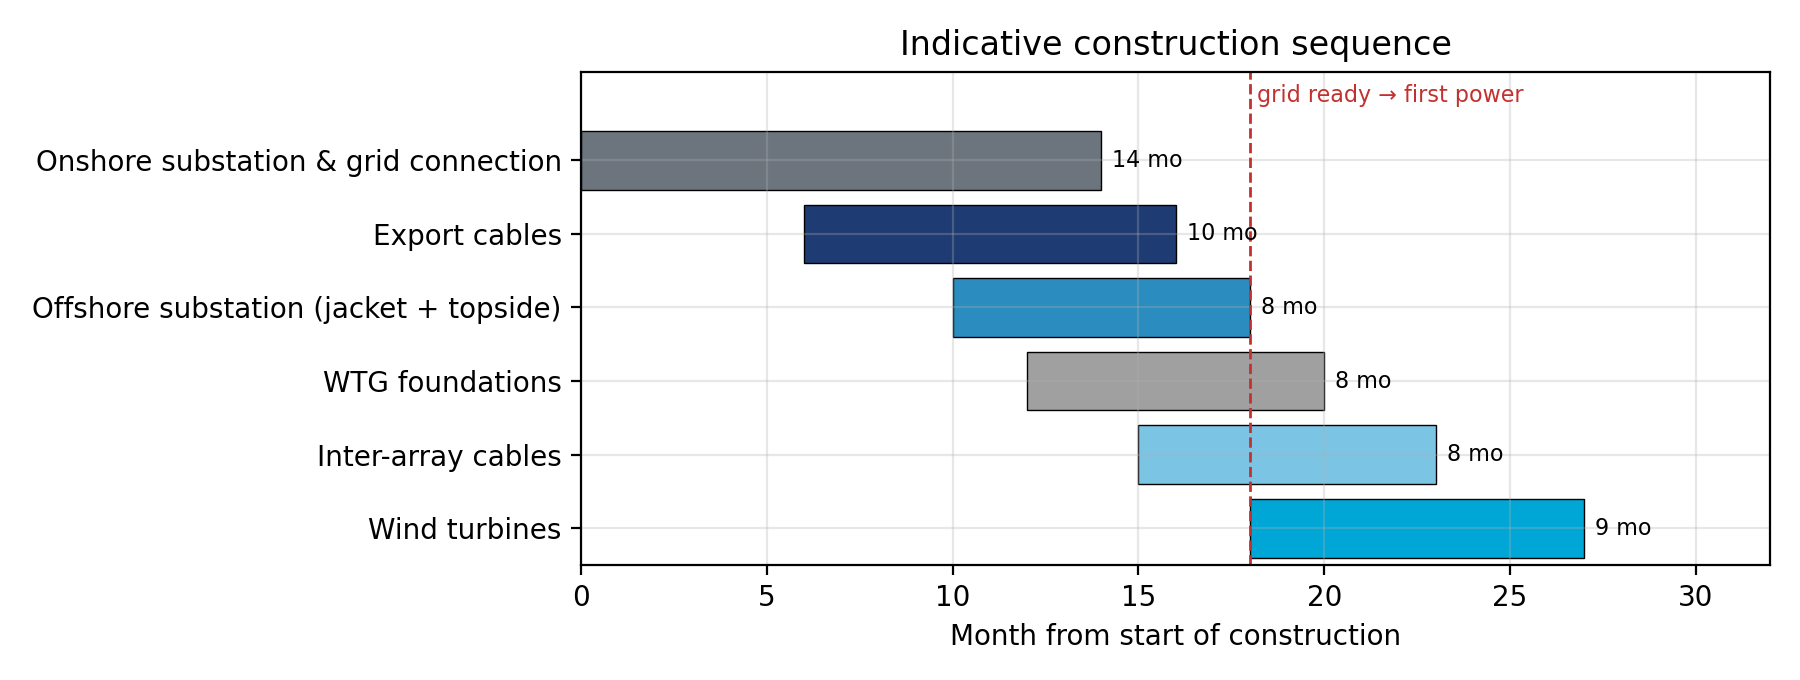
\includegraphics[width=0.8\textwidth]
    {figures/electrical/p4_construction_gantt.png}
    \caption{Indicative construction sequence: the grid connection and export system are ready when WTG installation starts.}
    \label{fig:elec-gantt}
\end{figure}

\begin{figure}[H]
    \centering
    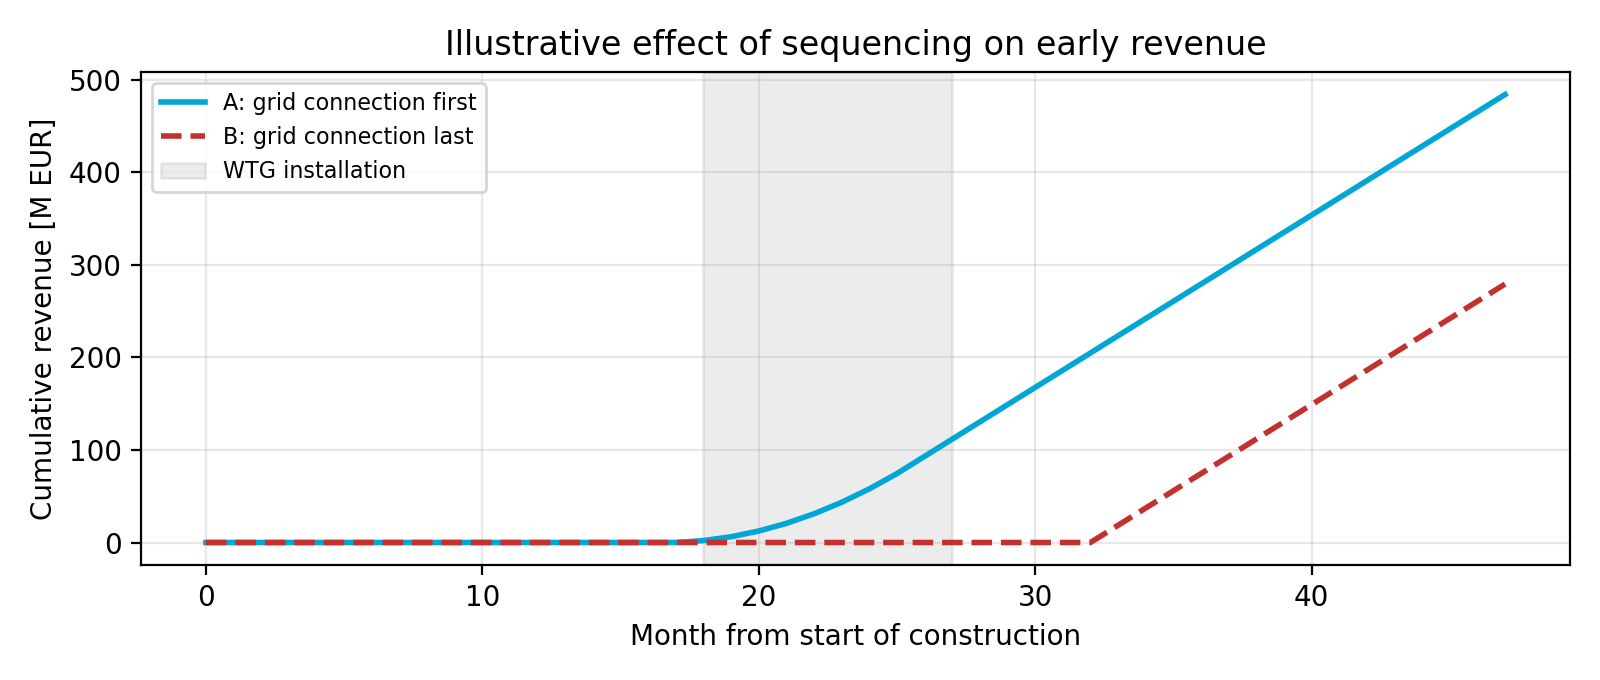
\includegraphics[width=0.7\textwidth]
    {figures/electrical/p4_revenue_sequence.png}
    \caption{Illustrative cumulative revenue for grid-first versus grid-last sequencing, using the same WTG installation campaign.}
    \label{fig:elec-revenue}
\end{figure}

\section{Feedback}
\label{sec:elec-feedback}
\begin{quote}
\emph{Offshore Renewable Technology is a new course. As your lecturers, we are motivated to learn with you and improve going forward. Therefore, we very much appreciate feedback on our work. Please provide your constructive feedback to the ORT-course thus far -- it can be on lectures, course material, assignments and you are also welcome to make suggestions. [1 pts]}
\end{quote}

% TODO (Group 21): adapt this draft to your own experience before submitting.
The lectures on electrical design connected theory and practice well. Real project examples, such as the Windpark Fryslân timeline from concept design to final design, made clear why choices about voltage level, number of export cables and redundancy are made. The Excel templates made the assignments concrete and easy to check step by step.

We have three suggestions. First, a short worked example of one row of the `IAC' tab during the lecture would make the expected method clearer, for example the role of $\cos\varphi$ and of the hours per bin. Second, some template cells contain fixed or rounded values, such as the hours of the first and last bin and the $21.1\,\mathrm{MVA}$ rating; a short note in the template would avoid confusion. Third, publishing all slides before the lecture, together with a list of the key formulas (three-phase power, losses, redundancy), would help us prepare for both the lectures and the exam.
.
%%  Change the title/subtitle in the template's title data to
%%  "Assignment 3" / "Electrical Aspects".
%%
%%  This file is only a standalone fallback that compiles the chapter with
%%  the TU Delft class if present, otherwise with the standard report class.
%% =====================================================================
\IfFileExists{tudelft-report.cls}{%
  \documentclass{tudelft-report}%
}{%
  \documentclass[11pt,a4paper]{report}%
  \usepackage[a4paper,margin=2.5cm]{geometry}%
}

\usepackage{amsmath}
\usepackage{graphicx}
\usepackage{float}
\usepackage{hyperref}

\title{Assignment 3}

\begin{document}

\begin{titlepage}
  \centering
  \vspace*{2cm}
  {\fontsize{40}{44}\selectfont Assignment 3\par}
  \vspace{0.8cm}
  {\LARGE Electrical Aspects\par}
  \vspace{1.2cm}
  {\small by\par}
  \vspace{1.2cm}
  {\LARGE Group 21\par}
  \vspace{1.2cm}
  \begin{tabular}{ll}
    Ameen, Amran            & 5578620 \\
    Chalkiadis, Theodoros   & 6537197 \\
    Schulze, Max            & 2723314 \\
  \end{tabular}
  \vfill
  \begin{flushleft}
  \begin{tabular}{ll}
    Instructors: & Dr.\ B.C.\ Ummels \\[4pt]
    Faculty:     & Faculty of Mechanical Engineering, Delft \\
  \end{tabular}
  \end{flushleft}
\end{titlepage}

\tableofcontents

\chapter{Electrical Aspects Assignment 3}
\label{ch:electrical}

% Structure follows 2026-10-07_ORT Assignment Wind+Electrical v.4.0.pdf
% (Parts 1--4 and Feedback). Each question is quoted before its answer.
% Input data: 2026-10-07_ORT Assignment Wind+Electrical.xlsx
% (tabs 'WTG Yield Wake' and 'IAC').
% All numerical results below were produced with the notebooks
% part1_grid_integration.ipynb, part2_iac_losses.ipynb,
% part3_electrical_design.ipynb and part4_development_construction.ipynb,
% and are reproduced here for the write-up. The completed IAC tab is in
% output/ORT_Assignment_Wind_Electrical_completed.xlsx.

\section{Grid Integration of Offshore Wind}
\label{sec:elec-part1}

\subsection{Turbine Data and Operational Areas}
\label{sec:elec-turbine}
The tab `WTG Yield Wake' of the supplied Excel file describes a $20\,\mathrm{MW}$ wind turbine generator (WTG) with a $280\,\mathrm{m}$ rotor at $160\,\mathrm{m}$ hub height, installed in a park of 80 WTGs. The swept area is $61{,}575\,\mathrm{m^2}$, giving a specific rating of $325\,\mathrm{W/m^2}$. The power coefficient follows from the template as

\begin{equation}
    C_P(v) = \frac{P(v)}{\tfrac{1}{2}\rho A v^3},
    \label{eq:elec-cp}
\end{equation}

with $\rho = 1.224\,\mathrm{kg/m^3}$. Figure~\ref{fig:elec-curves} shows the power curve, the thrust coefficient $C_T$ and $C_P$, together with the five operational areas of the assignment. Table~\ref{tab:elec-areas} lists how often each area occurs and what share of the energy it produces, using the wind speed distribution of the template. One WTG yields $98{,}815\,\mathrm{MWh/yr}$ (capacity factor $56.4\,\%$). The park including wakes yields $6503\,\mathrm{GWh/yr}$ (capacity factor $46.4\,\%$), so the overall wake loss is $17.7\,\%$.

\begin{figure}[H]
    \centering
    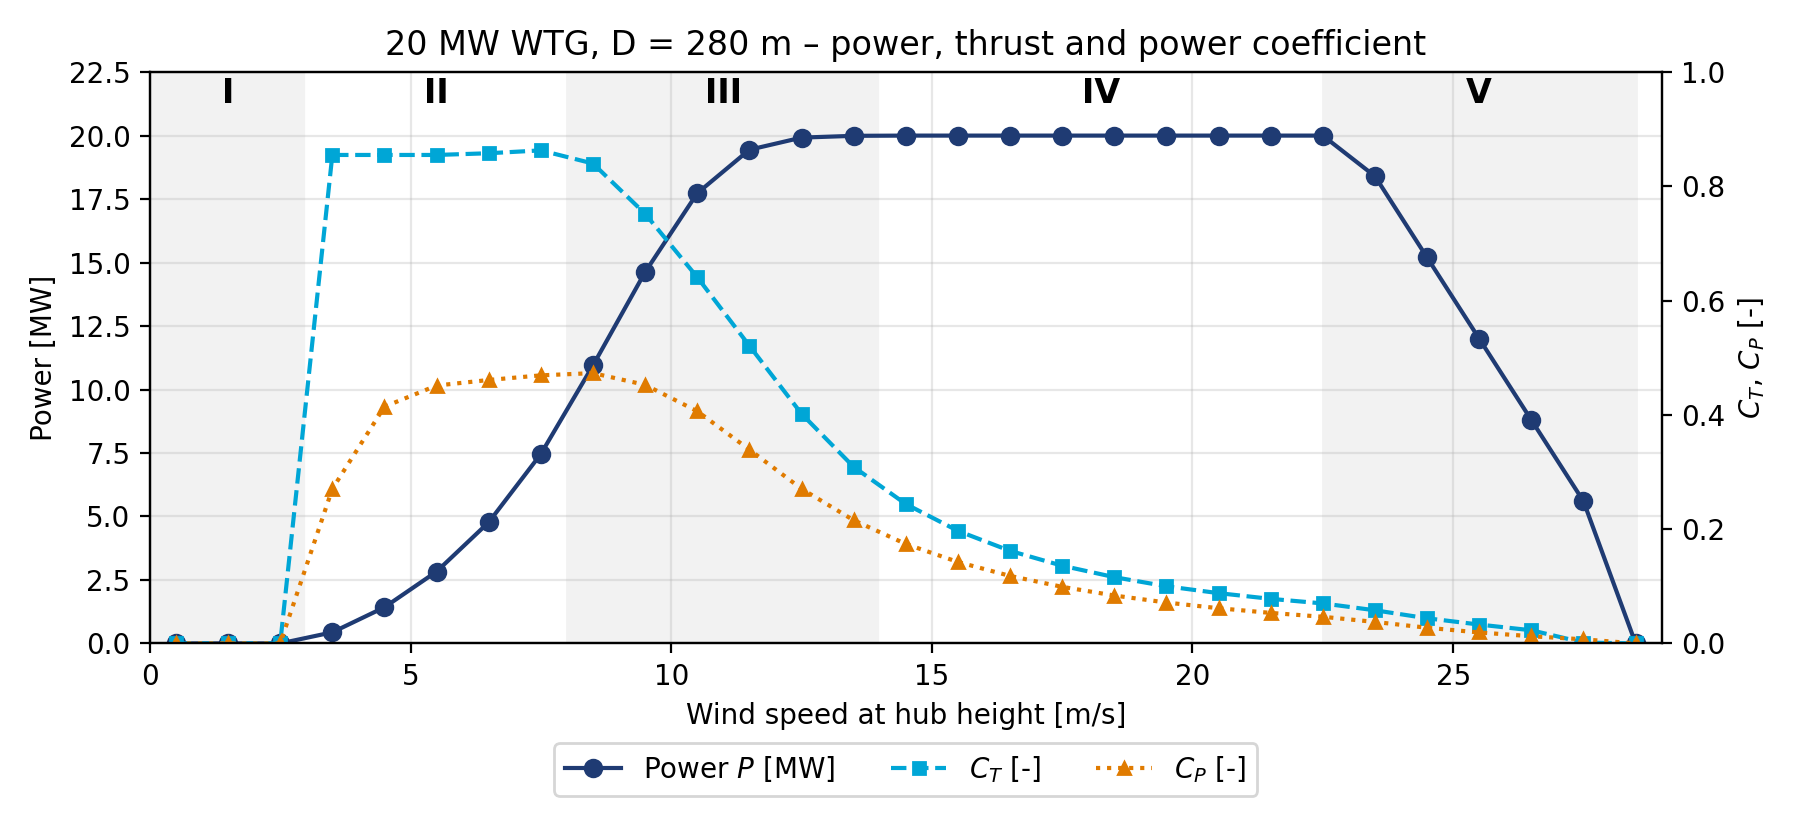
\includegraphics[width=0.85\textwidth]
    {figures/electrical/p1_power_thrust_areas.png}
    \caption{Power curve, thrust coefficient and power coefficient of the $20\,\mathrm{MW}$ WTG with operational areas I--V.}
    \label{fig:elec-curves}
\end{figure}

\begin{table}[H]
    \centering
    \caption{Operational areas, time share and share of the single-WTG energy yield.}
    \label{tab:elec-areas}
    \begin{tabular}{lcccc}
        \hline
        Area & Wind speed & Time & Hours & Energy \\
        & [m/s] & [\%] & [h/yr] & [\%] \\
        \hline
        I   & $< 3$       & 5.7  & 503   & 0.0  \\
        II  & 3 -- 8      & 37.1 & 3249  & 12.9 \\
        III & 8 -- 14     & 44.4 & 3892  & 64.7 \\
        IV  & 14 -- 22.5  & 12.1 & 1057  & 21.4 \\
        V   & 22.5 -- 28  & 0.7  & 63    & 1.1  \\
        \hline
    \end{tabular}
\end{table}

\subsection{Challenge of Operational Area I}
\label{sec:elec-area1}
\begin{quote}
\emph{What is the challenge of operational area I for the power balance in power systems? [1 pts]}
\end{quote}

In area I the wind speed is below cut-in, and the WTG produces no power at all. The grid still has to keep generation equal to load plus losses at every moment, so the whole load must then be covered by other sources: dispatchable plants, storage, demand response or imports. Low wind usually affects a whole region at once, so long calm periods hit all wind parks in that region together and do not average out. At this site area I occurs $5.7\,\%$ of the year (about $500\,\mathrm{h}$, Table~\ref{tab:elec-areas}). The challenge is that wind power adds almost no firm capacity. The system must keep nearly all of its conventional backup capacity available, even though that capacity runs only a few hours a year. Each time the wind crosses the cut-in speed, the park also switches between zero and some output, and the other units must follow these steps.

\subsection{Challenges of Operational Area III}
\label{sec:elec-area3}
\begin{quote}
\emph{What are two challenges of operational area III for keeping the power balance? [2 pts]}
\end{quote}

Area III (variable pitch, about $8$--$14\,\mathrm{m/s}$) is the steepest part of the power curve (Figure~\ref{fig:elec-dpdv}). It is also where the turbine runs most often ($44\,\%$ of the time) and where it produces most of its energy ($65\,\%$). This creates two challenges:

\begin{enumerate}
    \item \textbf{Large and fast power variations.} One WTG changes its output by up to $3.7\,\mathrm{MW}$ per $\mathrm{m/s}$ ($18\,\%$ of rated per $\mathrm{m/s}$). For the 80-WTG park, including wakes, this reaches about $255\,\mathrm{MW}$ per $\mathrm{m/s}$, or $16\,\%$ of installed capacity. Normal turbulence and passing weather fronts therefore cause large ramps. The system operator must balance these with fast reserves and the ramping ability of other units.
    \item \textbf{Amplified forecast errors.} Power is planned day-ahead and intraday from wind speed forecasts. In area III a forecast error of only $1\,\mathrm{m/s}$ becomes a power error of hundreds of MW for one park. The resulting imbalances must be covered by reserve capacity and cost balancing energy. In addition, the WTG runs at its maximum available power, so it can only regulate downwards. It cannot help to close a shortage unless it is curtailed beforehand.
\end{enumerate}

\begin{figure}[H]
    \centering
    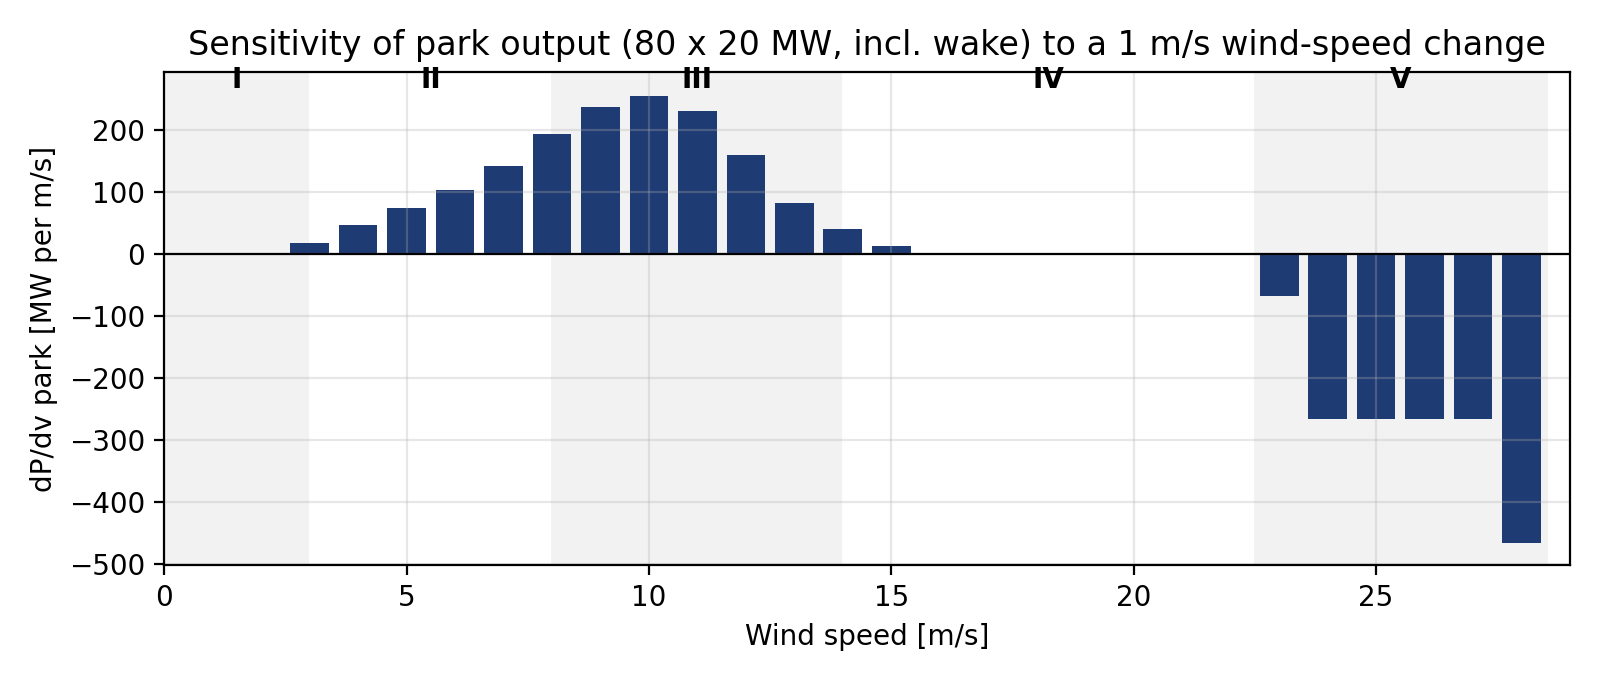
\includegraphics[width=0.8\textwidth]
    {figures/electrical/p1_sensitivity_dPdv.png}
    \caption{Change of park output for a $1\,\mathrm{m/s}$ change of wind speed (80 WTGs including wake).}
    \label{fig:elec-dpdv}
\end{figure}

\subsection{Area V versus a Hard Cut-Out}
\label{sec:elec-area5}
\begin{quote}
\emph{Older wind turbine types had a `hard cut-out' at a specific wind speed. The wind turbine would stop producing power when the wind speed would reach 25 m/s. It would start producing power again when the wind speed would have dropped at around 22 m/s. What are two benefits for power system operation of area V compared to a `hard cut-out' at a specific high wind speed, as is the case for older wind turbines? [2 pts]}
\end{quote}

To illustrate the difference, a synthetic storm passing over the 80-WTG park was simulated (Figure~\ref{fig:elec-storm}). The turbines see slightly different wind speeds, and each control strategy was applied to every turbine. Two benefits follow:

\begin{enumerate}
    \item \textbf{No sudden loss of a large block of generation.} With a hard cut-out, all WTGs in a park (and in neighbouring parks) stop within minutes once the storm passes $25\,\mathrm{m/s}$. For the system this is like the trip of a large power plant: frequency drops, and large, fast and expensive reserves are needed. In area V the output ramps down linearly between $22.5$ and $28\,\mathrm{m/s}$, so the park output falls gradually. In the simulation the largest 10-minute drop falls from about $700\,\mathrm{MW}$ (hard cut-out) to about $290\,\mathrm{MW}$ (area V) for the $1.6\,\mathrm{GW}$ park.
    \item \textbf{No hysteresis, so faster and more predictable recovery.} After a hard cut-out the WTG restarts only below $22\,\mathrm{m/s}$, so it stays off for hours while the wind would already allow production. Output then returns in large steps. In area V the turbine stays connected and follows the wind continuously. Its output is easier to forecast, it keeps supplying grid services such as reactive power and voltage control, and it avoids start/stop cycles. In the simulated storm the park produces about $15\,\%$ more energy ($48.4$ against $42.1\,\mathrm{GWh}$).
\end{enumerate}

\begin{figure}[H]
    \centering
    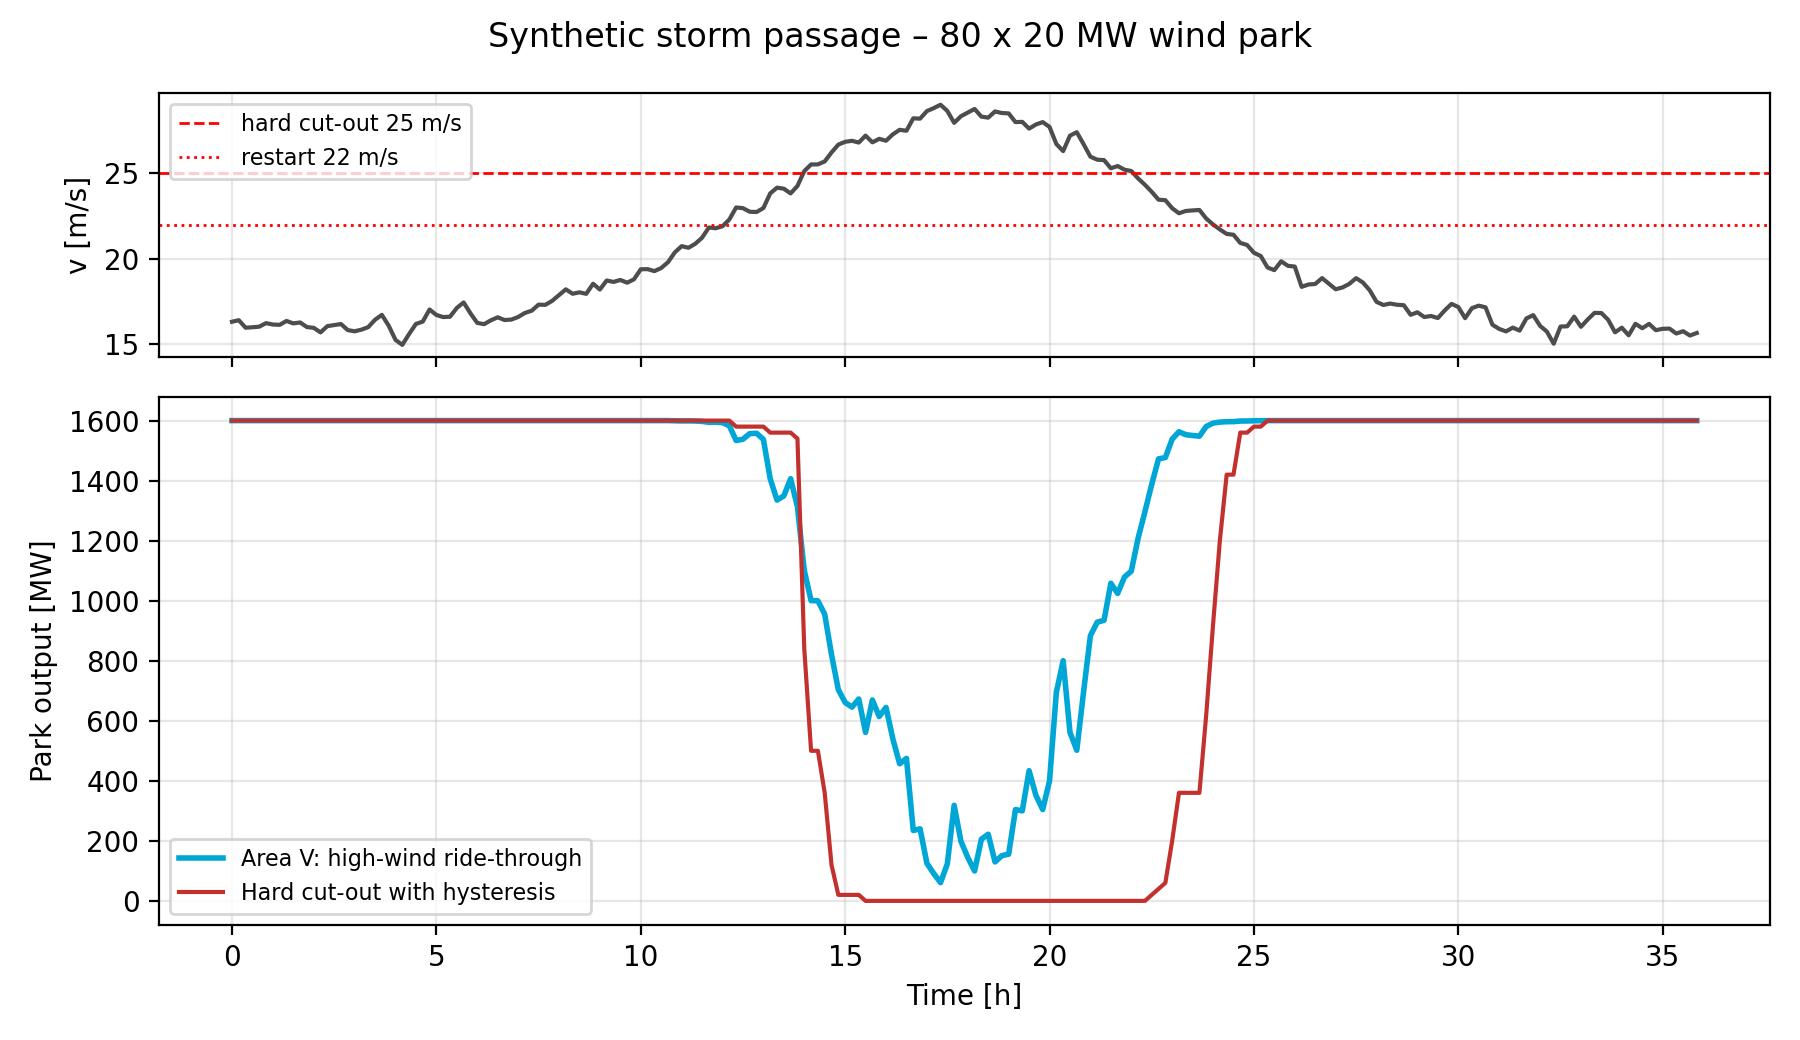
\includegraphics[width=0.85\textwidth]
    {figures/electrical/p1_storm_hwrt_vs_hardcutout.png}
    \caption{Synthetic storm passage: park output with high-wind ride-through (area V) and with a hard cut-out at $25\,\mathrm{m/s}$ and restart at $22\,\mathrm{m/s}$.}
    \label{fig:elec-storm}
\end{figure}

\subsection{Wind Speeds with Negligible Wake Effects}
\label{sec:elec-wake-negl}
\begin{quote}
\emph{Offshore wind parks consist of a cluster of wind turbines. The power production by such a cluster of wind turbines is dependent on the wake effects: the power production of wind turbines may be reduced in the wake of other turbines. In the Excel file, tab `WTG Yield Wake', an omni-directional wake effect for a wind park of 80 WTGs is provided for wind speeds at hub height. For this wind park, at what wind speeds are the wake effects negligible? [1 pts]}
\end{quote}

The wake effects are negligible between about $14.5$ and $22.5\,\mathrm{m/s}$, which is the rated-power range (area IV). The park efficiency is $99.2\,\%$ at $14.5\,\mathrm{m/s}$ and $99.94\,\%$ from $15.5$ to $22.5\,\mathrm{m/s}$, a loss of only $0.06\,\%$ (Figure~\ref{fig:elec-eta}). Above $22.5\,\mathrm{m/s}$ the wake even increases production (Section~\ref{sec:elec-wake-high}). Below $14\,\mathrm{m/s}$ the losses are significant.

\begin{figure}[H]
    \centering
    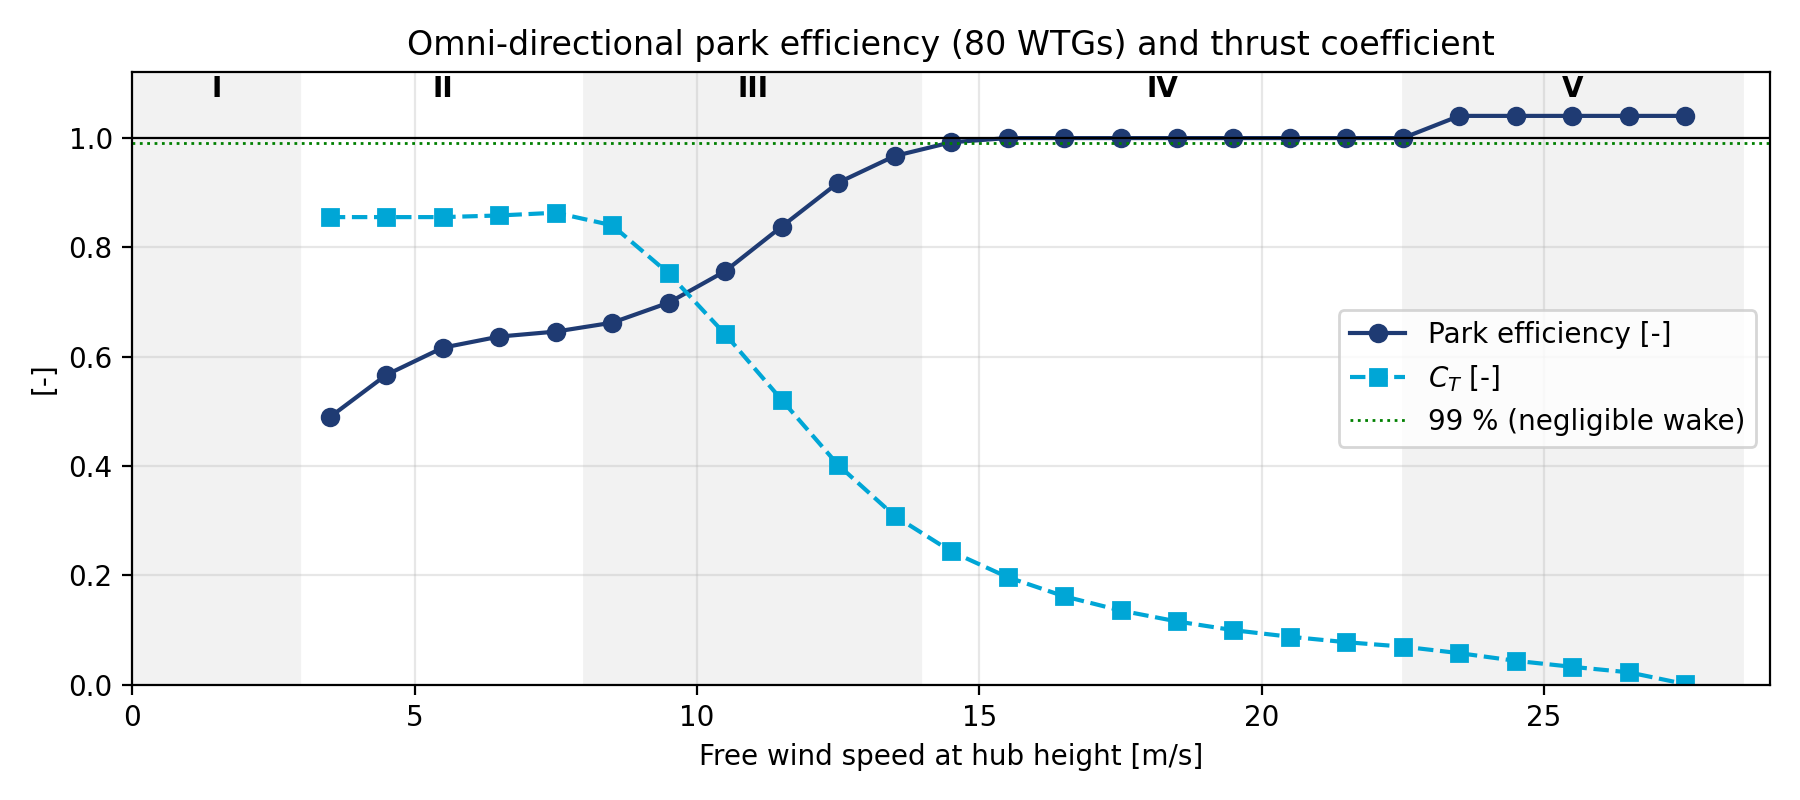
\includegraphics[width=0.85\textwidth]
    {figures/electrical/p1_park_efficiency_ct.png}
    \caption{Omni-directional park efficiency of the 80-WTG park and thrust coefficient versus free wind speed.}
    \label{fig:elec-eta}
\end{figure}

\subsection{Wake Impact in Areas II, III and IV}
\label{sec:elec-wake-areas}
\begin{quote}
\emph{Explain for operational areas II, III and IV what impact the wake effects have on power production of an offshore wind park. Consider the thrust curve as part of your answer. [2 pts]}
\end{quote}

The velocity deficit in a wake grows with the thrust coefficient. Just behind the rotor, momentum theory gives

\begin{equation}
    \frac{u_{wake}}{u_\infty} \approx \sqrt{1 - C_T},
    \label{eq:elec-wake}
\end{equation}

so a WTG that takes more momentum out of the flow leaves a slower wake. Table~\ref{tab:elec-wakeareas} quantifies the impact per area.

\begin{itemize}
    \item \textbf{Area II} ($3$--$8\,\mathrm{m/s}$): $C_T$ is high and nearly constant ($\approx 0.86$), so the wake deficit is largest. Power scales with $v^3$, so a waked WTG loses a large share of its output. The park efficiency is only $49$--$65\,\%$. The power levels are low, so the absolute loss ($375\,\mathrm{GWh/yr}$) is about $27\,\%$ of the total wake loss.
    \item \textbf{Area III} ($8$--$14\,\mathrm{m/s}$): the blades pitch and $C_T$ falls from $0.84$ to about $0.3$. The wake deficit therefore decreases, and the park efficiency rises from $66\,\%$ to $97\,\%$. However, this area holds most of the energy and the power curve is steepest here, so even a small deficit costs a lot of power. Area III causes about $73\,\%$ of the wake losses ($1025\,\mathrm{GWh/yr}$). In effect, the wakes shift the park power curve to higher wind speeds, so the park reaches rated power later than a single WTG.
    \item \textbf{Area IV} ($14$--$22.5\,\mathrm{m/s}$): $C_T$ is low ($<0.25$), so the wakes are weak. Even a waked WTG still sees a wind speed above rated and keeps producing $20\,\mathrm{MW}$. The wake loss is negligible ($4.6\,\mathrm{GWh/yr}$).
\end{itemize}

\begin{table}[H]
    \centering
    \caption{Annual gross and net (including wake) park production per operational area.}
    \label{tab:elec-wakeareas}
    \begin{tabular}{lcccc}
        \hline
        Area & Gross & Net & Wake loss & Share of wake loss \\
        & [GWh/yr] & [GWh/yr] & [GWh/yr] & [\%] \\
        \hline
        II  & 1017.0 & 642.3  & 374.8  & 26.7 \\
        III & 5111.0 & 4086.2 & 1024.8 & 73.1 \\
        IV  & 1691.5 & 1686.9 & 4.6    & 0.3  \\
        V   & 85.7   & 87.4   & $-1.8$ & $-0.1$ \\
        \hline
        Total & 7905.2 & 6502.8 & 1402.4 & 100 \\
        \hline
    \end{tabular}
\end{table}

\subsection{Wake Benefit at Very High Wind Speeds}
\label{sec:elec-wake-high}
\begin{quote}
\emph{At high wind speeds (23.5 -- 27.5 m/s), the wake effect slightly increases power production of the wind park as a whole, compared to an individual wind turbine. Provide a technical explanation for this effect of wind park wakes. In your answer, consider that wake involves a lower wind speed behind a wind turbine and consider the power curve of the turbine at that wind speed range. [1 pts]}
\end{quote}

Between $22.5$ and $28\,\mathrm{m/s}$ (area V) the power curve has a negative slope of about $-3.2\,\mathrm{MW}$ per $\mathrm{m/s}$: the WTG reduces its output as the wind speed rises, to limit loads. A WTG in the wake of another turbine sees a lower wind speed than the free stream, so it operates higher on this descending part of the curve and produces more. For example, a free-stream WTG at $24.5\,\mathrm{m/s}$ produces $15.2\,\mathrm{MW}$, while a waked WTG that sees $23.5\,\mathrm{m/s}$ produces $18.4\,\mathrm{MW}$. Some downstream turbines may even stay below $22.5\,\mathrm{m/s}$ and produce rated power. $C_T$ is very small at these wind speeds ($<0.06$), so the deficits are small and the net gain is limited to about $4\,\%$ (park efficiency $1.04$).

\subsection{Opportunities of a Larger Rotor for the Owner}
\label{sec:elec-rotor-owner}
\begin{quote}
\emph{In the past decade, wind turbines have become much larger. This is true for the generator sizes [MW], but even more for the rotor diameters [m] which have become larger also relative to generator size. Compare two identical wind turbines with a fixed capacity [MW] but with different rotor sizes. Discuss two opportunities of a larger wind turbine rotor for the owner of a wind park. Include the operational areas of relevance in your answer. [2 pts]}
\end{quote}

To quantify the effect, the same $20\,\mathrm{MW}$ generator was combined with a $236\,\mathrm{m}$ rotor ($457\,\mathrm{W/m^2}$) and a $280\,\mathrm{m}$ rotor ($325\,\mathrm{W/m^2}$). Both use the same aerodynamic $C_P$ curve, the same high-wind control and the same wind distribution (Figure~\ref{fig:elec-rotor}, Table~\ref{tab:elec-rotor}). The model is simplified: it uses $C_{P,max}=0.47$ up to rated power, so the absolute yields differ slightly from the template.

\begin{enumerate}
    \item \textbf{More energy and a higher capacity factor (areas II and III).} The captured power scales with the swept area, $P \propto D^2 v^3$. The larger rotor therefore produces more at every wind speed below rated and reaches rated power at a lower wind speed ($10.5$ instead of $12.5\,\mathrm{m/s}$). Area III shifts to lower wind speeds and area IV becomes wider. The annual yield rises by about $16\,\%$ (capacity factor $49.8\,\% \rightarrow 57.9\,\%$), and the hours at rated power rise from about $2000$ to $3300\,\mathrm{h/yr}$.
    \item \textbf{Better use of the expensive electrical system and higher revenue per MWh.} The generator, converter, inter-array cables, substation and export cables are sized on MW, not on rotor size. A larger rotor sends more MWh through the same electrical infrastructure, which lowers the levelised cost of energy and the grid connection cost per MWh. Most of the extra energy is produced at low to moderate wind speeds (areas II and III). In those hours total wind production in the market is lower, so electricity prices are usually higher and the market value per MWh improves.
\end{enumerate}

The trade-offs are higher rotor loads, larger foundations and stronger wakes, which require a larger turbine spacing.

\begin{figure}[H]
    \centering
    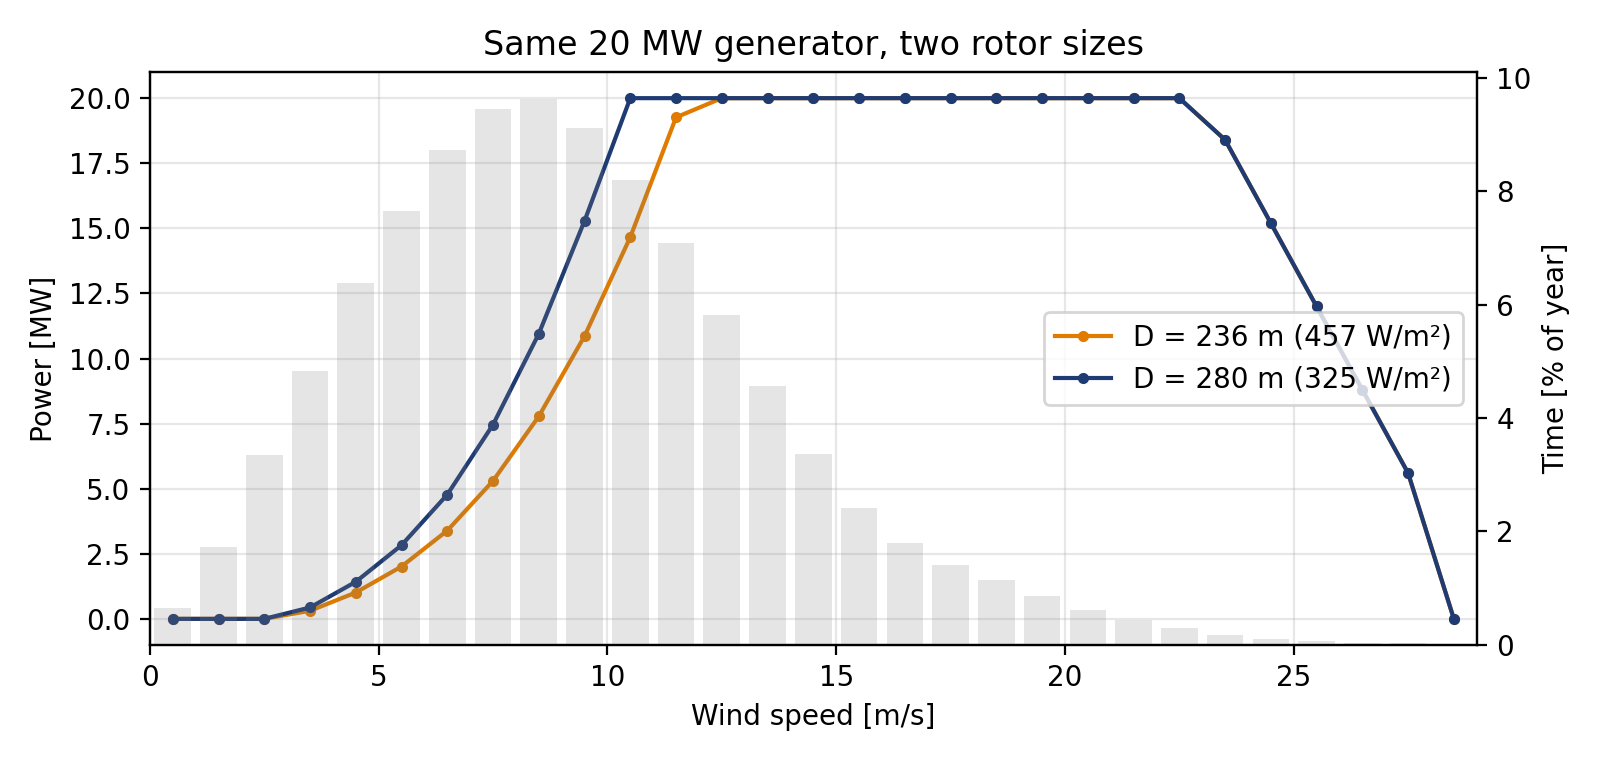
\includegraphics[width=0.75\textwidth]
    {figures/electrical/p1_rotor_size_comparison.png}
    \caption{Power curves of a $20\,\mathrm{MW}$ WTG with a $236\,\mathrm{m}$ and a $280\,\mathrm{m}$ rotor, with the wind speed distribution of the template.}
    \label{fig:elec-rotor}
\end{figure}

\begin{table}[H]
    \centering
    \caption{Comparison of two rotor sizes for the same $20\,\mathrm{MW}$ generator (simplified model).}
    \label{tab:elec-rotor}
    \begin{tabular}{lcc}
        \hline
        Quantity & $D=236\,\mathrm{m}$ & $D=280\,\mathrm{m}$ \\
        \hline
        Specific rating [$\mathrm{W/m^2}$] & 457 & 325 \\
        Rated power reached at [m/s] & 12.5 & 10.5 \\
        Annual energy yield [MWh/yr] & 87,179 & 101,366 \\
        Capacity factor [\%] & 49.8 & 57.9 \\
        Hours at rated power [h/yr] & 1993 & 3332 \\
        Maximum $dP/dv$ [MW per m/s] & 4.60 & 4.71 \\
        Mean $|\Delta P|$ for a $1\,\mathrm{m/s}$ forecast error [MW] & 1.68 & 1.74 \\
        \quad relative to mean output [\%] & 16.9 & 15.0 \\
        Standard deviation / mean of output [-] & 0.76 & 0.67 \\
        \hline
    \end{tabular}
\end{table}

\subsection{A Larger Rotor from a Power System Perspective}
\label{sec:elec-rotor-system}
\begin{quote}
\emph{Argue if a larger rotor could be beneficial from a power system operation point of view. Consider variations of the power produced and wind forecast errors in your answer. [2 pts]}
\end{quote}

On balance, a larger rotor (lower specific rating) benefits power system operation.

Regarding variations of the power produced, the WTG reaches rated power at a lower wind speed, so it spends far more time in area IV ($67\,\%$ more hours at rated). In area IV, wind fluctuations do not change the output at all. Output in low winds is also higher, so there are fewer hours near zero. The production profile becomes flatter and more like baseload: relative variability (standard deviation divided by mean) drops from $0.76$ to $0.67$, and the capacity factor rises, so the grid connection is used better. One drawback is that the steep part of the curve (area III) moves to $7$--$10\,\mathrm{m/s}$, the most frequent wind speeds, so ramps occur in more common weather conditions.

Regarding wind forecast errors, a forecast error has no effect on power in area IV, and the larger rotor widens this area. More hours of the year are therefore insensitive to forecast errors. In absolute terms the expected power error for a $1\,\mathrm{m/s}$ forecast error is almost unchanged ($1.68$ against $1.74\,\mathrm{MW}$). Relative to the higher mean output it is lower ($16.9\,\% \rightarrow 15.0\,\%$), so each MWh delivered needs less balancing reserve.

A larger rotor therefore gives a smoother, more predictable and firmer supply per MW of grid capacity. The main side effect is more hours with high wind output at moderate wind speeds. In systems with a very high wind share, this can increase curtailment or the number of hours with low or negative prices.

\section{Inter-Array Cabling Losses}
\label{sec:elec-part2}

\subsection{Cable Data}
\label{sec:elec-cable-data}
The three inter-array cable (IAC) types of the assignment are listed in Table~\ref{tab:elec-cables}. The WTGs are $20\,\mathrm{MW}$ units operating at $\cos\varphi = 0.95$. Wake losses are neglected, which gives a conservative (high) estimate of the cable currents.

\begin{table}[H]
    \centering
    \caption{Inter-array cable types at $66\,\mathrm{kV}$ and resulting maximum number of $20\,\mathrm{MW}$ WTGs.}
    \label{tab:elec-cables}
    \begin{tabular}{lcccccc}
        \hline
        Cable & Type & Ampacity & $R$ & Ampacity$/I_{WTG}$ & $n_{max}$ & Loading at $n_{max}$ \\
        & [$\mathrm{mm^2}$] & [A] & [$\Omega$/km] & [-] & [-] & [\%] \\
        \hline
        Cable 1 & 400 & 424 & 0.101 & 2.30 & 2 & 86.9 \\
        Cable 2 & 630 & 584 & 0.063 & 3.17 & 3 & 94.6 \\
        Cable 3 & 800 & 750 & 0.037 & 4.07 & 4 & 98.2 \\
        \hline
    \end{tabular}
\end{table}

\subsection{Rated Current per Wind Turbine}
\label{sec:elec-current}
\begin{quote}
\emph{The type indicates the cross-section of the aluminium conductor [mm$^2$]. The ampacity is the maximum current [A] the cable type is designed to handle. Assume you are using 20 MW offshore wind turbines. For the calculation, assume that every wind turbine operates at cos $\varphi$ = 0.95 and do not consider any wake losses (conservative estimate for the current in the cables). Calculate the rated current per wind turbine. [2 pts]}
\end{quote}

The apparent power of one WTG is

\begin{equation}
    S_{WTG} = \frac{P}{\cos\varphi} = \frac{20\,\mathrm{MW}}{0.95} = 21.05\,\mathrm{MVA}.
    \label{eq:elec-swtg}
\end{equation}

With the three-phase relation $S = \sqrt{3}\,U_{ph-ph}\,I$, the rated current at $66\,\mathrm{kV}$ is

\begin{equation}
    I_{WTG} = \frac{S_{WTG}}{\sqrt{3}\,U} = \frac{21.05\times10^{6}\,\mathrm{VA}}{\sqrt{3}\cdot 66\times10^{3}\,\mathrm{V}} = 184.2\,\mathrm{A}.
    \label{eq:elec-iwtg}
\end{equation}

The template rounds the WTG rating to $21.1\,\mathrm{MVA}$, which gives $184.6\,\mathrm{A}$. That value is used in the `IAC' tab.

\subsection{Maximum Number of WTGs per Cable Type}
\label{sec:elec-nmax}
\begin{quote}
\emph{Determine the maximum number of wind turbines that can be connected to Cable 1, Cable 2 and Cable 3 without exceeding the ampacity. [2 pts]}
\end{quote}

The maximum number of WTGs per cable is

\begin{equation}
    n_{max} = \left\lfloor \frac{I_{ampacity}}{I_{WTG}} \right\rfloor,
    \label{eq:elec-nmax}
\end{equation}

which gives $424/184.2 = 2.30$, so \textbf{2 WTGs} on Cable 1 ($368\,\mathrm{A}$); $584/184.2 = 3.17$, so \textbf{3 WTGs} on Cable 2 ($552\,\mathrm{A}$); and $750/184.2 = 4.07$, so \textbf{4 WTGs} on Cable 3 ($737\,\mathrm{A}$), as summarised in Table~\ref{tab:elec-cables}.

\subsection{Annual IAC Losses of the String}
\label{sec:elec-iac-losses}
\begin{quote}
\emph{Assume that you want to use the cheapest cable type where possible. Review the Excel file, tab `IAC' and, using your answers above, complete all yellow cells. What is the annual electricity loss as a percentage of the yield of the WTGs on the string? [2 pts]}
\end{quote}

The string in the `IAC' tab connects four WTGs. Each cable section is named after the WTG at its upstream end and carries the power of all WTGs before it. For each section, the cheapest (smallest) cable whose ampacity is not exceeded was selected. Table~\ref{tab:elec-yellow} shows the completed yellow cells.

\begin{table}[H]
    \centering
    \caption{Completed yellow cells of the `IAC' tab (rows 11--13).}
    \label{tab:elec-yellow}
    \begin{tabular}{lcccc}
        \hline
        Section & WTG 1 & WTG 2 & WTG 3 & WTG 4 \\
        \hline
        Number of WTGs on IAC section & 1 & 2 & 3 & 4 \\
        Section length [km] & 2.5 & 2.5 & 2.0 & 1.5 \\
        Nominal current [A] (E11:H11) & 184.6 & 369.2 & 553.7 & 738.3 \\
        IAC cable (E12:H12) & 1 & 1 & 2 & 3 \\
        Resistance [$\Omega$/km] (E13:H13) & 0.101 & 0.101 & 0.063 & 0.037 \\
        Loading [\%] & 43.5 & 87.1 & 94.8 & 98.4 \\
        \hline
    \end{tabular}
\end{table}

Column D (rows 18--46) holds the apparent power per wind speed bin, $S(v) = P(v)/0.95$. The loss in section $k$ follows the template formula, in which the current scales with the actual output:

\begin{equation}
    P_{loss,k}(v) = 3\left(\frac{S(v)}{S_{nom}}\,I_{nom,k}\right)^2 R_k L_k.
    \label{eq:elec-ploss}
\end{equation}

Multiplying by the hours in each bin and summing over all bins and sections gives the annual string losses (cell K48) of $1341.6\,\mathrm{MWh/yr}$. The energy yield of the four WTGs (cell K49) is

\begin{equation}
    E_{string} = 4\sum_{v} P(v)\,h(v) = 394{,}990\,\mathrm{MWh/yr},
    \label{eq:elec-yield}
\end{equation}

so the annual loss (cell K50) is

\begin{equation}
    \frac{E_{loss}}{E_{string}} = \frac{1341.6}{394{,}990} = 0.34\,\%.
    \label{eq:elec-losspct}
\end{equation}

The annual IAC loss is therefore \textbf{0.34\,\% of the WTG yield}. At full power the instantaneous loss is $334\,\mathrm{kW}$ ($0.42\,\%$ of $80\,\mathrm{MW}$). The annual percentage is lower because losses scale with $I^2$ and the WTGs run below rated most of the time. Sections 3 and 4, which carry the highest currents, cause the largest losses (Figure~\ref{fig:elec-iac}).

\begin{figure}[H]
    \centering
    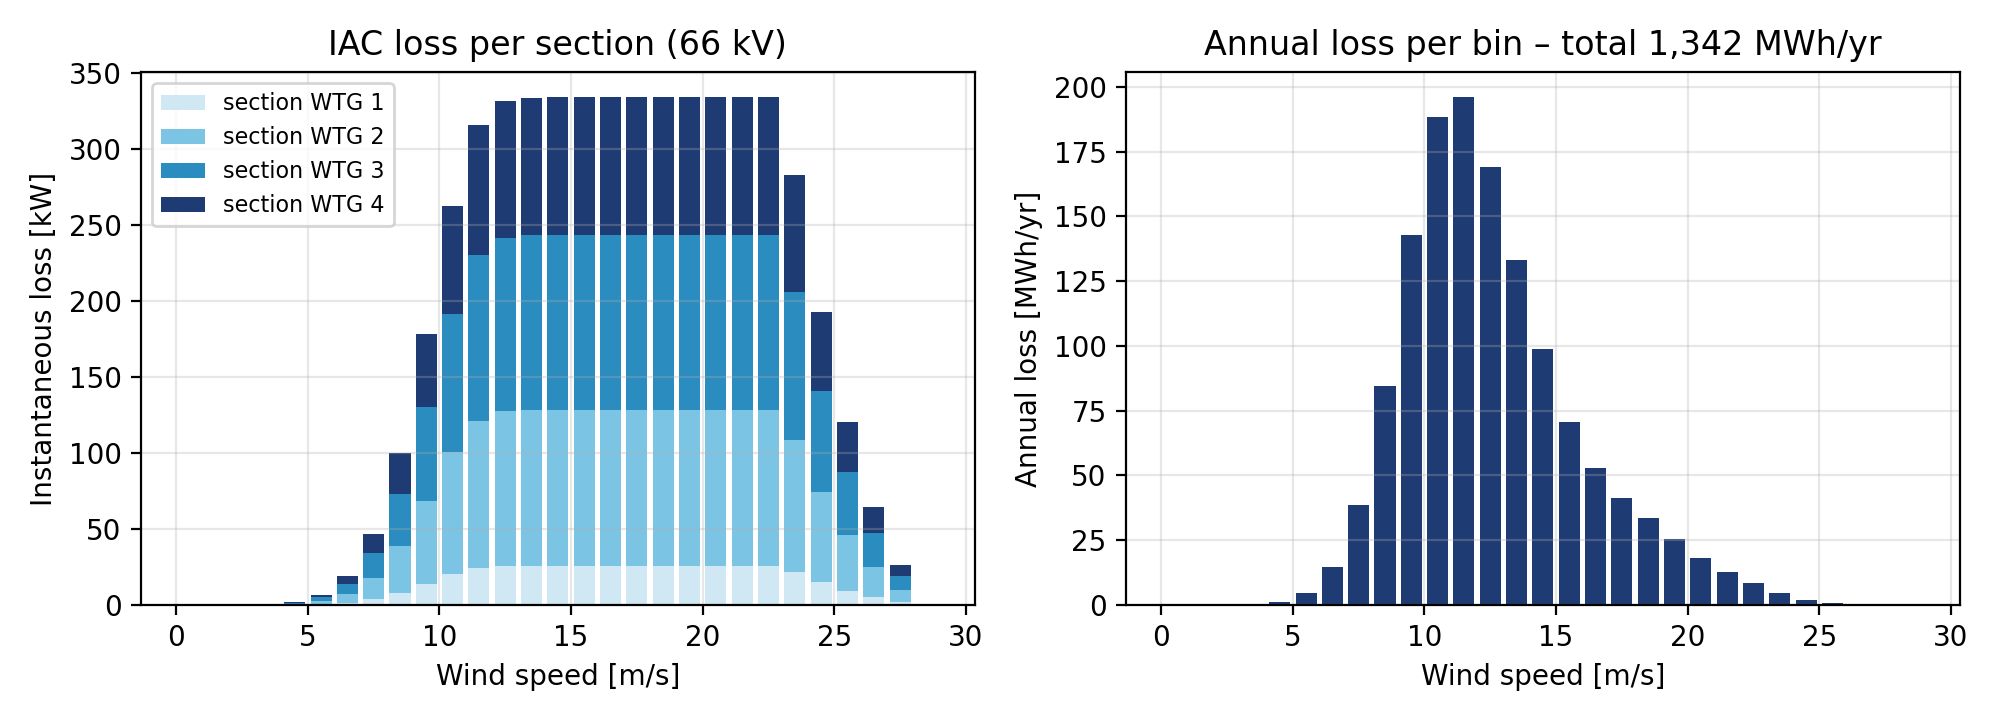
\includegraphics[width=\textwidth]
    {figures/electrical/p2_iac_losses.png}
    \caption{Left: instantaneous IAC losses per string section versus wind speed at $66\,\mathrm{kV}$. Right: annual losses per wind speed bin.}
    \label{fig:elec-iac}
\end{figure}

\subsection{Number of WTGs on Cable 1 at 132 kV}
\label{sec:elec-132-n}
\begin{quote}
\emph{Assume that the voltage level of the cables would be 132 kV instead of 66 kV and that the conductor resistance would be the same. How many WTGs of 20 MW could be connected to Cable 1 if it would be at 132 kV? [1 pt]}
\end{quote}

Doubling the voltage halves the current per WTG:

\begin{equation}
    I_{WTG,132} = \frac{21.05\,\mathrm{MVA}}{\sqrt{3}\cdot 132\,\mathrm{kV}} = 92.1\,\mathrm{A},
    \qquad \frac{424}{92.1} = 4.60.
    \label{eq:elec-i132}
\end{equation}

At $132\,\mathrm{kV}$, Cable 1 can therefore connect \textbf{4 WTGs} ($80\,\mathrm{MW}$, $368\,\mathrm{A}$), twice as many as at $66\,\mathrm{kV}$.

\subsection{Loss Reduction at 132 kV}
\label{sec:elec-132-loss}
\begin{quote}
\emph{How much would the annual losses on the wind turbine string be reduced if the voltage level would be increased to 132 kV, everything else being equal? Explain your answer. [1 pt]}
\end{quote}

The power is the same, so $S = \sqrt{3}UI$ gives half the current at twice the voltage. Ohmic losses scale with the square of the current, $P_{loss} = 3I^2R$. With the same cables (same $R$ and $L$),

\begin{equation}
    \frac{P_{loss,132}}{P_{loss,66}} = \left(\frac{66}{132}\right)^2 = \frac{1}{4}.
    \label{eq:elec-lossratio}
\end{equation}

The annual losses drop by \textbf{75\,\%}, from $1341.6\,\mathrm{MWh/yr}$ ($0.34\,\%$) to $335.4\,\mathrm{MWh/yr}$ ($0.085\,\%$), a saving of about $1006\,\mathrm{MWh/yr}$ per string. This is why array systems have moved from $33$ to $66\,\mathrm{kV}$ and now to $132\,\mathrm{kV}$: a higher voltage means a lower current and lower losses. At $132\,\mathrm{kV}$ the cheaper Cable 1 could also be used for the whole string. The losses would then be $562\,\mathrm{MWh/yr}$, still $58\,\%$ lower than the $66\,\mathrm{kV}$ base case, at a lower cable cost. In return, the higher voltage requires more expensive switchgear and WTG transformers with a higher insulation level.

\section{Offshore Wind Park Electrical Design}
\label{sec:elec-part3}

\subsection{Single-Line Diagram}
\label{sec:elec-sld}
The single-line diagram (Figure~\ref{fig:elec-sld}) shows 12 strings in six pairs. Each pair connects 11 WTGs of $12\,\mathrm{MVA}$ ($132\,\mathrm{MVA}$) to one $66\,\mathrm{kV}$ busbar section, which feeds one secondary winding of a $220/66/66\,\mathrm{kV}$ transformer. The installed wind power is $66 \times 12\,\mathrm{MVA} = 792\,\mathrm{MVA}$. The substation has three transformers rated $264/132/132\,\mathrm{MVA}$ (ONAN) and $400/200/200\,\mathrm{MVA}$ (ONAF), and three $220\,\mathrm{kV}$ export cables, one per transformer bay. Both the $66\,\mathrm{kV}$ and the $220\,\mathrm{kV}$ busbars have bus-section couplers.

\begin{figure}[H]
    \centering
    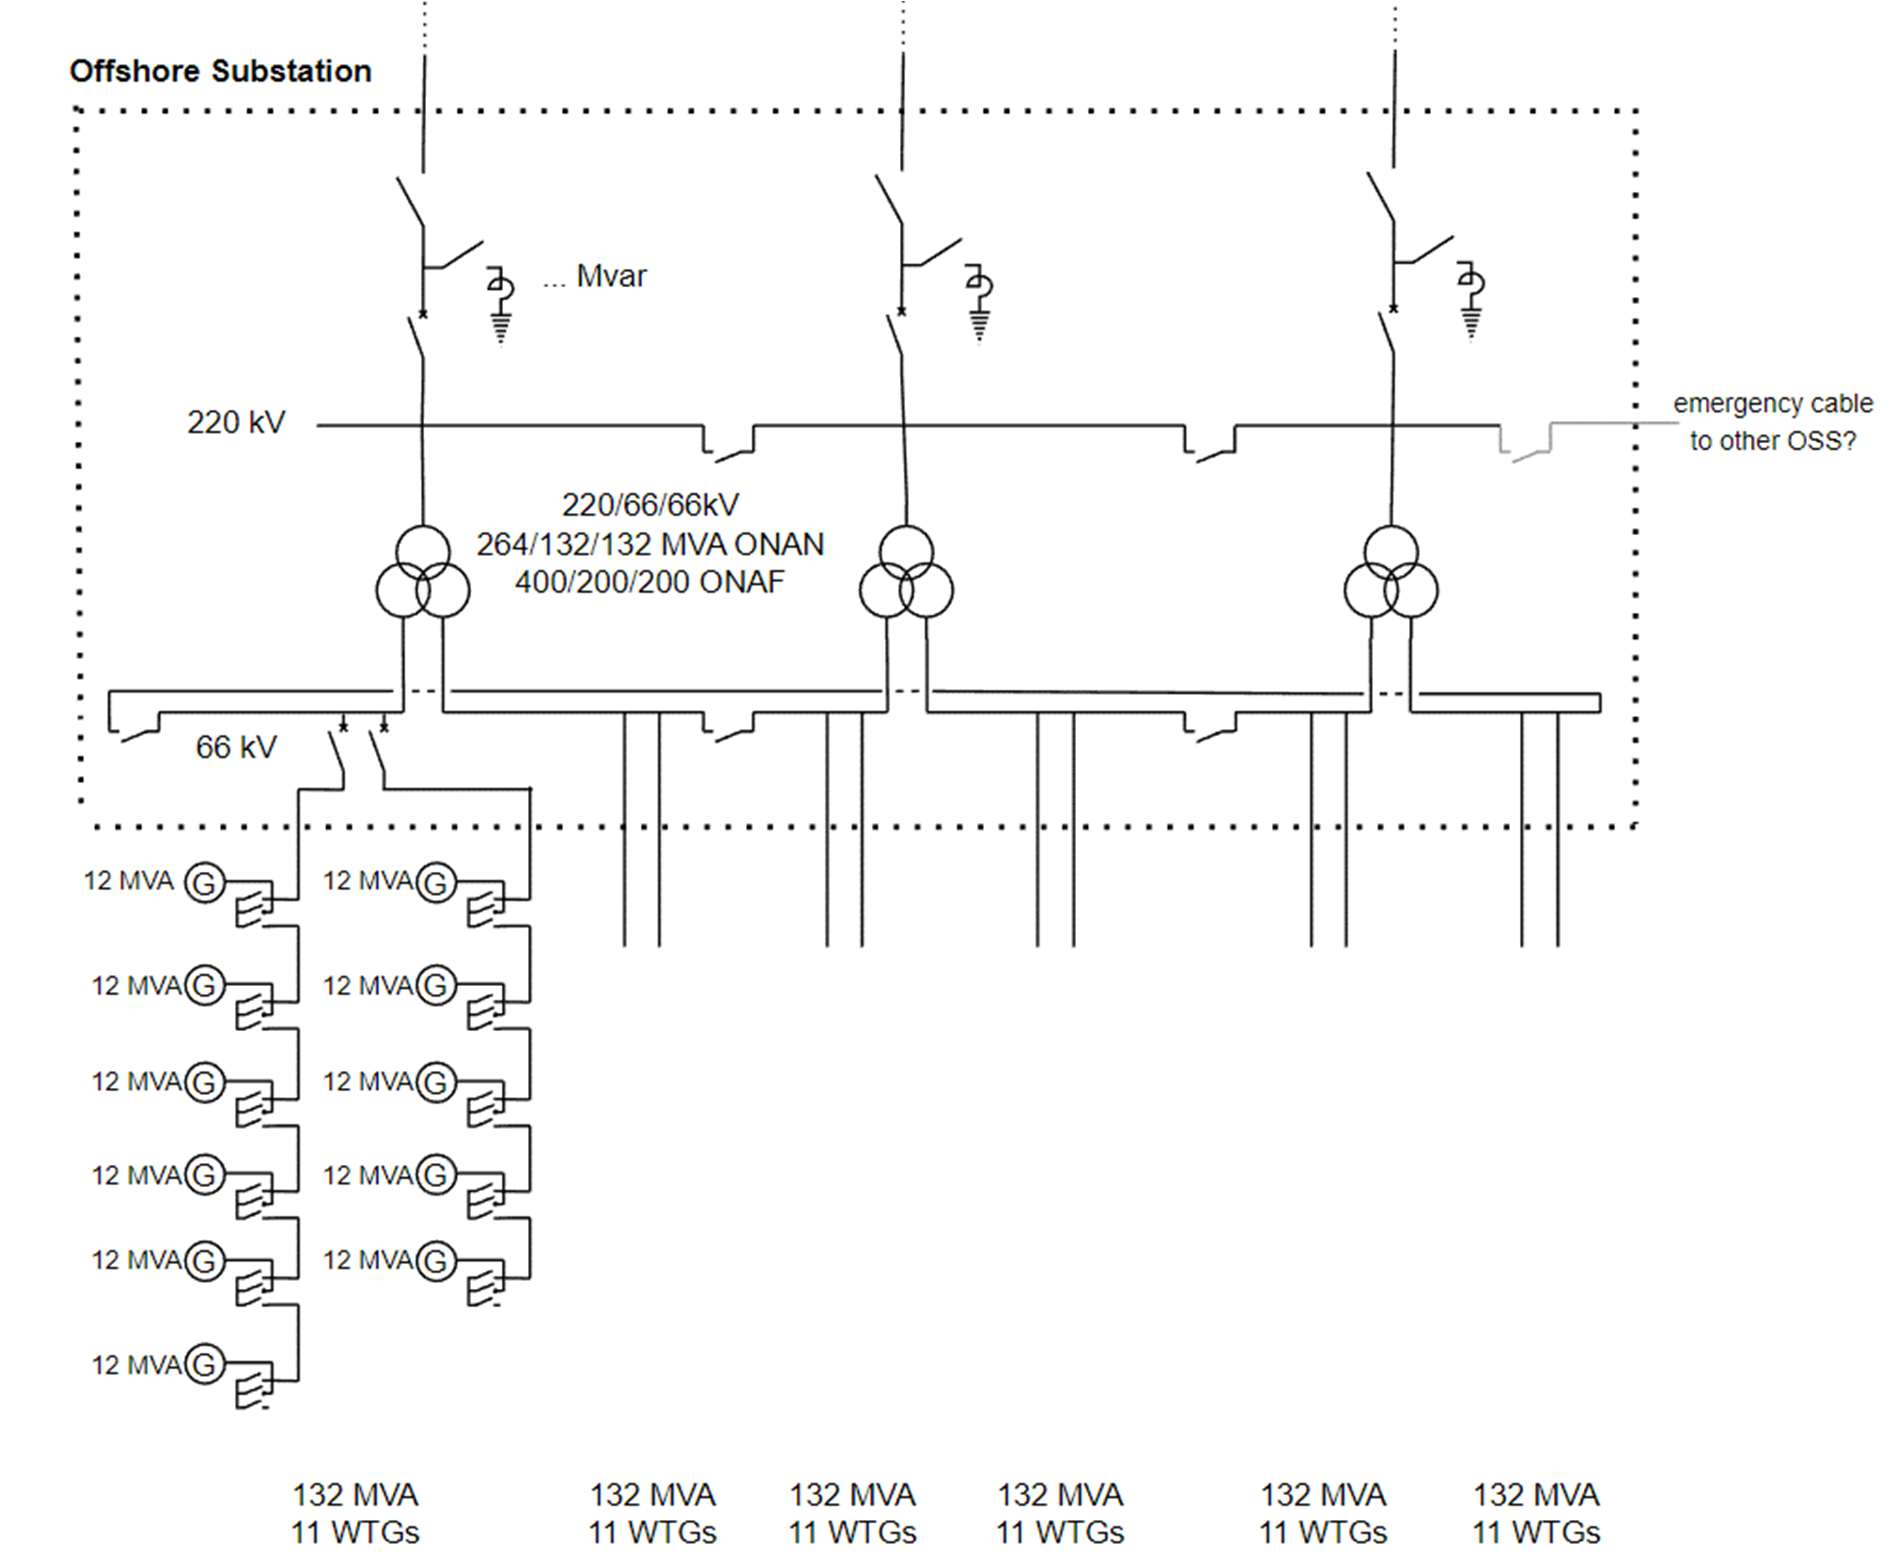
\includegraphics[width=0.85\textwidth]
    {figures/electrical/given_single_line_diagram.png}
    \caption{Single-line diagram of the offshore substation, as given in the assignment (only two of the twelve strings are drawn).}
    \label{fig:elec-sld}
\end{figure}

\subsection{Power over One Export Cable}
\label{sec:elec-export-power}
\begin{quote}
\emph{For normal operation, how much power would flow over one export cable? [1 pts]}
\end{quote}

In normal operation the three transformers and three export cables share the park output equally:

\begin{equation}
    S_{cable} = \frac{66 \times 12\,\mathrm{MVA}}{3} = \frac{792\,\mathrm{MVA}}{3} = 264\,\mathrm{MVA}.
    \label{eq:elec-scable}
\end{equation}

Each export cable therefore carries \textbf{264\,MVA}, equal to the ONAN rating of one transformer. This corresponds to a current of $264\,\mathrm{MVA}/(\sqrt{3}\cdot 220\,\mathrm{kV}) = 693\,\mathrm{A}$. Collection-system losses and reactive power are neglected.

\subsection{Transformer Winding Currents}
\label{sec:elec-winding}
\begin{quote}
\emph{For normal operation, how much current is flowing on one 66 kV winding of the transformer? How much current is flowing on the 220 kV winding of the transformer? [2 pts]}
\end{quote}

Each $66\,\mathrm{kV}$ winding is fed by one busbar section with 11 WTGs ($132\,\mathrm{MVA}$), and the $220\,\mathrm{kV}$ winding carries the sum of both secondary windings ($264\,\mathrm{MVA}$):

\begin{equation}
    I_{66} = \frac{132\,\mathrm{MVA}}{\sqrt{3}\cdot 66\,\mathrm{kV}} = 1155\,\mathrm{A},
    \qquad
    I_{220} = \frac{264\,\mathrm{MVA}}{\sqrt{3}\cdot 220\,\mathrm{kV}} = 693\,\mathrm{A}.
    \label{eq:elec-iwinding}
\end{equation}

As a check, $2 \times 1155 / 693 = 3.33 = 220/66$. The current ratio equals the voltage ratio, so power is conserved over the transformer.

\subsection{Redundancy of the Offshore Transformers}
\label{sec:elec-redundancy}
\begin{quote}
\emph{For this exercise, redundancy can be assumed to be the \% of the installed wind power [MVA] over the installed transformer power [MVA]. Assume that there is emergency operation because one of the three transformers has an electrical fault and is out of service (N-1). Assume that all wind turbines are available for power production and the substation has been set so that all wind turbines are connected to the remaining two transformers. What is the level of redundancy [\%] when considering the offshore substation transformers? Support your answer using a short calculation. [2 pts]}
\end{quote}

With one transformer out of service, the two remaining units run at their ONAF (emergency) rating of $400\,\mathrm{MVA}$:

\begin{equation}
    \text{Redundancy} = \frac{S_{wind}}{S_{TR,available}} = \frac{792\,\mathrm{MVA}}{2 \times 400\,\mathrm{MVA}} = \frac{792}{800} = 99\,\%.
    \label{eq:elec-redundancy}
\end{equation}

Each remaining transformer carries $396\,\mathrm{MVA}$ ($1039\,\mathrm{A}$ at $220\,\mathrm{kV}$). Each $66\,\mathrm{kV}$ winding carries $198\,\mathrm{MVA}$ ($1732\,\mathrm{A}$), against its $200\,\mathrm{MVA}$ ONAF rating. The two transformers can therefore export the full park output with $1\,\%$ ($8\,\mathrm{MVA}$) margin, without curtailment, so the transformer design is fully N-1 redundant. Without forced cooling (ONAN) the ratio would be $792/528 = 150\,\%$, and one third of the park would have to be curtailed. Table~\ref{tab:elec-red} compares all cases.

\begin{table}[H]
    \centering
    \caption{Installed wind power versus available transformer capacity.}
    \label{tab:elec-red}
    \begin{tabular}{lcccc}
        \hline
        Case & Transformers & Capacity & Wind/capacity & Margin \\
        & [-] & [MVA] & [\%] & [MVA] \\
        \hline
        Normal, ONAN & 3 & 792  & 100 & 0 \\
        Normal, ONAF & 3 & 1200 & 66  & 408 \\
        N-1, ONAN    & 2 & 528  & 150 & $-264$ \\
        N-1, ONAF    & 2 & 800  & 99  & 8 \\
        \hline
    \end{tabular}
\end{table}

\subsection{Optimal Capacity of the Export Cable Circuits}
\label{sec:elec-export-capacity}
\begin{quote}
\emph{What would be the optimal capacity [MVA] of the export cable circuits? [2 pts]}
\end{quote}

The optimal capacity is about \textbf{264\,MVA per export circuit}, or roughly $700\,\mathrm{A}$ at $220\,\mathrm{kV}$. Three circuits then give $3 \times 264 = 792\,\mathrm{MVA}$, equal to the installed wind power. Three arguments support this choice:

\begin{itemize}
    \item \textbf{A transformer outage does not overload the cables.} The $220\,\mathrm{kV}$ busbar has bus-section couplers. During the N-1 transformer case, the $792\,\mathrm{MVA}$ from the two remaining transformers is spread over all three export cables, so each still carries $264\,\mathrm{MVA}$. A $400\,\mathrm{MVA}$ cable rating, matching the ONAF transformer rating, would only be needed if each cable were tied to its own transformer.
    \item \textbf{Oversizing the cables costs more than it saves.} Export cables are among the most expensive components, and their cost rises with conductor cross-section and installation effort. Sizing every cable for $400\,\mathrm{MVA}$ would only pay off during rare cable outages. If one of three cables is lost, $2 \times 264 = 528\,\mathrm{MVA}$ remains. According to the park duration curve (Figure~\ref{fig:elec-duration}), this still carries the full output $62\,\%$ of the time and $83\,\%$ of the energy during such an outage. The cheap redundancy is in the transformers (fans for ONAF), not in the cables.
    \item \textbf{Undersizing loses energy permanently.} For example, with $3 \times 200\,\mathrm{MVA}$ the park would be curtailed in every high-wind hour and lose about $11\,\%$ of its yield.
\end{itemize}

In practice a small margin above $264\,\mathrm{MVA}$ is chosen. The cable must also carry reactive current: its charging current is only partly compensated by the shunt reactors in the single-line diagram, and the grid code requires reactive power exchange. It must also operate at the lowest allowed voltage. The thermal time constant of the cable allows short overloads.

\begin{figure}[H]
    \centering
    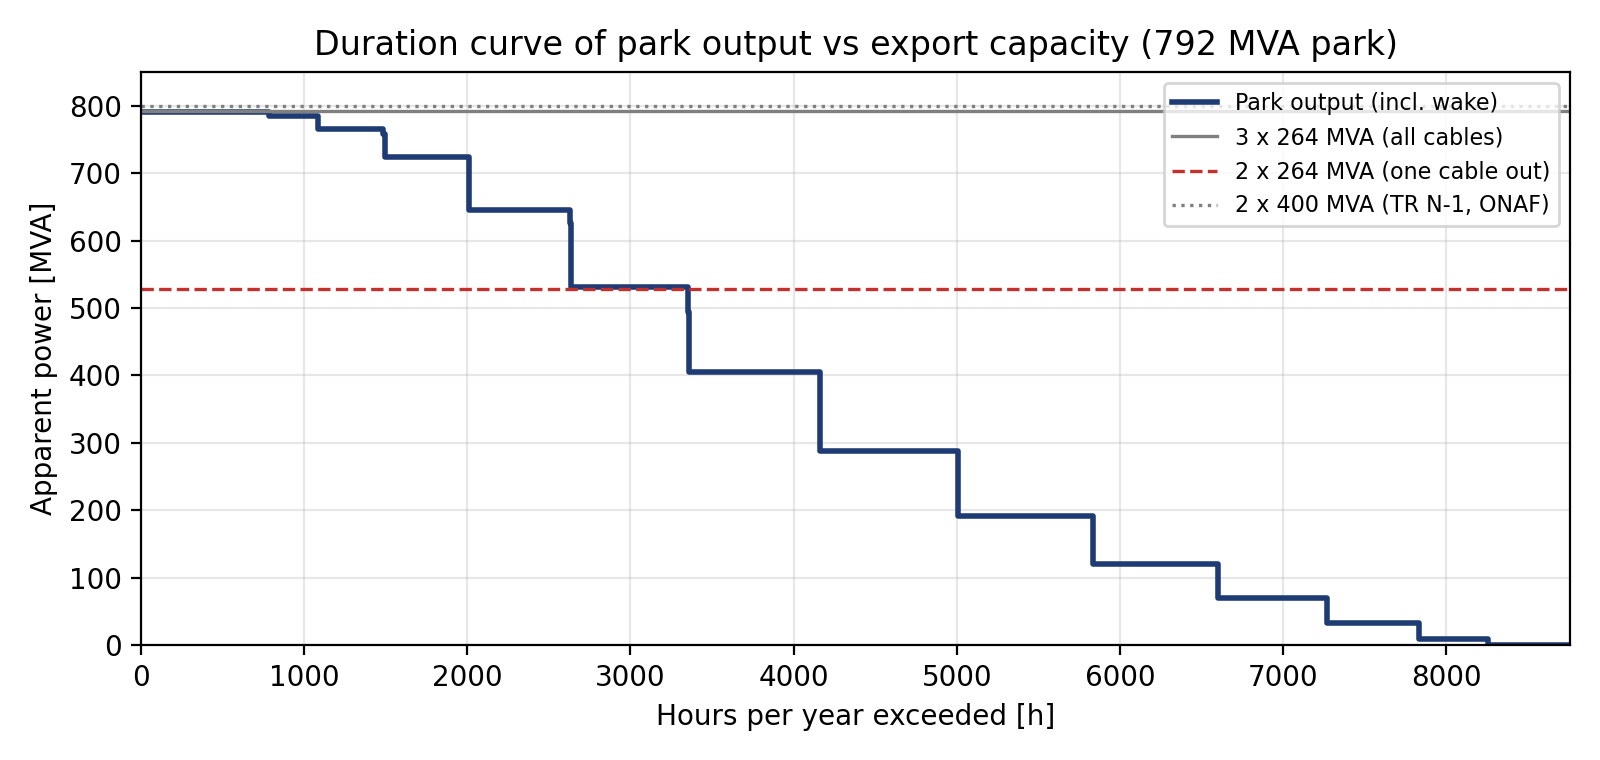
\includegraphics[width=0.75\textwidth]
    {figures/electrical/p3_duration_export_capacity.png}
    \caption{Duration curve of the park output (template wind distribution including wake, scaled to $792\,\mathrm{MVA}$) and export capacity for different cable configurations.}
    \label{fig:elec-duration}
\end{figure}

\subsection{Emergency Connection to Another Substation}
\label{sec:elec-emergency}
\begin{quote}
\emph{On the right in the single-line diagram, an option is indicated for an emergency connection to another substation. The emergency cable cannot be used to export wind power, but it can keep the substation and the wind turbines energized in case all export cables to shore would be out of service. Discuss three factors that you would consider in your decision to build that connection or not. [3 pts]}
\end{quote}

\begin{enumerate}
    \item \textbf{Probability and consequence of losing all export cables.} Three independent circuits rarely fail together, but common-mode failures are possible: a shared cable corridor or landfall (anchor drag, fishing, dredging), a fault in the onshore substation, or a grid outage. Repairing an export cable can take months because of vessel availability and winter weather. Without power the WTGs and the offshore substation lose their auxiliary supply. There is then no heating or dehumidification, which causes condensation and corrosion in converters, switchgear and nacelles. The turbines cannot yaw during storms, which raises loads. SCADA stops working, and the legally required aviation and navigation lights go out. The longer the expected outage, the more valuable the emergency link.
    \item \textbf{Cost of the link versus alternatives.} The link needs an extra cable, a switchgear bay with protection at both ends, installation and possibly cable crossings. The alternative is diesel generators on the substation, plus UPS systems in the WTGs. The auxiliary demand of this park is only about $2$--$3\,\mathrm{MW}$ (assuming about $30\,\mathrm{kW}$ per WTG). A 60-day outage would need about $3.3\,\mathrm{GWh}$, roughly EUR 1.3 million of offshore diesel, plus fuel logistics, emissions and generator maintenance. The emergency cable can be small (a few MVA plus charging current), so its cost depends mainly on the distance to the other substation.
    \item \textbf{Technical and organisational feasibility.} Several conditions must be checked: there must be a neighbouring substation within a reasonable distance, at the same voltage level, with spare capacity, and able to supply the charging current (reactive power) of the link. Protection must stay selective, so that a fault or disturbance cannot spread from one park to the other. Ownership must also be settled. The other substation may belong to another developer or to the transmission system operator (TSO), which requires agreements on operation, liability and cost sharing. The link also has extra benefits. During construction it can energise the park for commissioning before the export cables are finished, and later it can become part of a meshed offshore grid that increases availability.
\end{enumerate}

\section{Offshore Wind Park Development and Construction}
\label{sec:elec-part4}

\subsection{Project Context}
\label{sec:elec-context}
\begin{quote}
\emph{You are asked to develop a new offshore wind project that will be visible from land. The project is developed in a country that does not have offshore wind yet. Although there is general support for offshore wind, your project may face opposition from different stakeholders. The different stakeholders include: 1) the national government, 2) the local government, 3) a nature conservation society, 4) local fishermen, 5) the local port, 6) the grid company that will connect the wind park.}
\end{quote}

The project is the first offshore wind project in the country and is visible from land. Most stakeholder risks therefore come from uncertainty and novelty, and most opportunities come from starting a new industry.

\subsection{Risks and Opportunities per Stakeholder}
\label{sec:elec-stakeholders}
\begin{quote}
\emph{For each stakeholder, list a possible risk that your project may pose for the stakeholder. [2 pts]}
\end{quote}
\begin{quote}
\emph{For each stakeholder, list a possible gain or opportunity that your project could provide. [2 pts]}
\end{quote}

Table~\ref{tab:elec-stakeholders} lists one main risk and one main gain or opportunity for each stakeholder.

\begin{table}[H]
    \centering
    \caption{Possible risks and gains or opportunities of the project for each stakeholder.}
    \label{tab:elec-stakeholders}
    \small
    \begin{tabular}{p{0.17\textwidth}p{0.37\textwidth}p{0.37\textwidth}}
        \hline
        Stakeholder & Possible risk & Possible gain / opportunity \\
        \hline
        National government & Political and reputational risk if the first project is delayed, over budget or meets public resistance; fiscal risk if a subsidy is required. & Contribution to climate and renewable energy targets, energy security and less import dependence; start of a national offshore wind industry. \\
        \hline
        Local government & Visual impact on the coastline and possible effect on tourism and property values; nuisance from the onshore cable route and substation works. & Local jobs and tax income, a community fund, upgraded port and grid infrastructure, image as a green region. \\
        \hline
        Nature conservation society & Bird and bat collisions, underwater noise during pile driving (marine mammals), habitat disturbance from cables and scour protection. & Artificial reef effect and nature-inclusive design, a no-trawling zone acting as a marine protected area, monitoring data, replacement of fossil generation. \\
        \hline
        Local fishermen & Loss of fishing grounds and longer sailing routes; risk of gear snagging on cables; reduced catch during construction. & Compensation, guard-vessel and survey contracts, passive fishing or aquaculture inside the park, higher fish stocks near the foundations. \\
        \hline
        Local port & Congestion and conflicts with existing users; investment in quays and storage areas that may not pay back if no follow-up projects come. & Marshalling and O\&M base for decades: new revenue, jobs and a position as offshore wind hub for future projects. \\
        \hline
        Grid company (TSO) & Grid congestion and balancing effort due to variable output; required onshore reinforcements; technical risk of a first offshore connection. & Large new generation close to the coast, experience with offshore grid standards, possible reuse of the substation as a future grid hub. \\
        \hline
    \end{tabular}
\end{table}

\subsection{Developer Strategy}
\label{sec:elec-strategy}
\begin{quote}
\emph{Shortly describe a strategy for you as the project developer to minimize these risks and maximize these opportunities. [2 pts]}
\end{quote}

The strategy is early, transparent and continuous stakeholder engagement, combined with benefit sharing and mitigation by design:

\begin{itemize}
    \item \textbf{Engage early and openly.} Map the stakeholders before the site and layout are fixed. Hold public consultations with photomontages from the coast, appoint a fisheries liaison officer, and set up regular meetings with the municipality, the port and the TSO. Concerns raised early can still change the design (layout, distance from the coast, cable route), which builds trust.
    \item \textbf{Mitigate the main impacts by design.} Base the environmental impact assessment on solid baseline surveys. Use noise mitigation during piling (bubble curtains, soft-start, seasonal windows), curtail turbines during bird migration, bury cables deep enough and share as-built data with fishermen, and use nature-inclusive scour protection. Comply with the grid code (fault and high-wind ride-through, reactive power) and agree a staggered energisation plan with the TSO.
    \item \textbf{Share the benefits.} Set up a community fund or local co-ownership. Contract local vessels for guard, survey and crew-transfer work, and compensate fishermen. Sign a long-term marshalling and O\&M contract with the port so that its investment pays back. Offer the national government open data and lessons learned, so that this first project becomes the reference for the national offshore wind programme.
    \item \textbf{Secure the grid connection and permits early}, so that lead times and requirements are known and all stakeholders see a credible and reliable project.
\end{itemize}

\subsection{Construction Sequence}
\label{sec:elec-construction}
\begin{quote}
\emph{You have managed your stakeholders well and you have a permit to build the project. The construction of the project will consist of different phases. Argue in what order the phases should be to make the project as profitable as possible. Describe what your decision is based on [3 pts]: the wind turbines; the offshore substation; the onshore substation with the grid connection; the wind turbine foundations; the inter-array cables between the wind turbines; the export cables between the offshore and the onshore substation.}
\end{quote}

The proposed order is shown in Figure~\ref{fig:elec-gantt}:

\begin{enumerate}
    \item \textbf{Onshore substation with grid connection.} This phase has the longest lead time (power transformers, onshore permits, grid reinforcements by the TSO), and the work is onshore with little weather risk.
    \item \textbf{Export cables} between the onshore and offshore substations.
    \item \textbf{Offshore substation} (jacket and topside), energised from shore through the export cables.
    \item \textbf{WTG foundations.} This phase can start in parallel with steps 2--3 as soon as vessels and weather windows allow, because it does not depend on the grid.
    \item \textbf{Inter-array cables}, pulled in string by string behind the foundation campaign and connected to the energised offshore substation.
    \item \textbf{Wind turbines}, installed last on the finished foundations, so that each WTG produces power as soon as it is commissioned.
\end{enumerate}

This order is based on the following considerations:

\begin{itemize}
    \item \textbf{Early revenue and the time value of money.} The WTGs are the largest investment and the only part that earns money. If the full electrical chain (grid connection, export cable, substation, IAC) is ready before the first WTG is installed, every WTG produces as soon as it is commissioned. This gives first power during the installation campaign and shortens the time between spending capital and earning revenue. In the illustrative case of Figure~\ref{fig:elec-revenue} ($792\,\mathrm{MW}$, capacity factor $46\,\%$, EUR 70/MWh, $7\,\%$ discount rate), finishing the grid connection 6 months after the turbines instead of before them costs about EUR 175 million of discounted revenue.
    \item \textbf{Physical dependencies and the critical path.} The foundations must come before the IAC and the WTGs. The IAC needs the J-tubes on the foundations and the substation as its end point. Commissioning a WTG requires power from the grid. The onshore and export works have the longest lead times, so they start first.
    \item \textbf{Asset protection.} Installed but unpowered WTGs and cables need diesel generators for heating and dehumidification, or they risk corrosion damage. Energising the electrical system first avoids this.
    \item \textbf{Weather windows and vessel availability.} Pile driving and turbine lifting need calm summer windows and specialised vessels. Running the foundation campaign in parallel with the electrical works keeps these campaigns in the right season. The Windpark Fryslân timeline from the lecture follows the same logic: export cables and substation in 2019, foundations and IAC in 2020, and IAC and WTGs in 2021.
\end{itemize}

\begin{figure}[H]
    \centering
    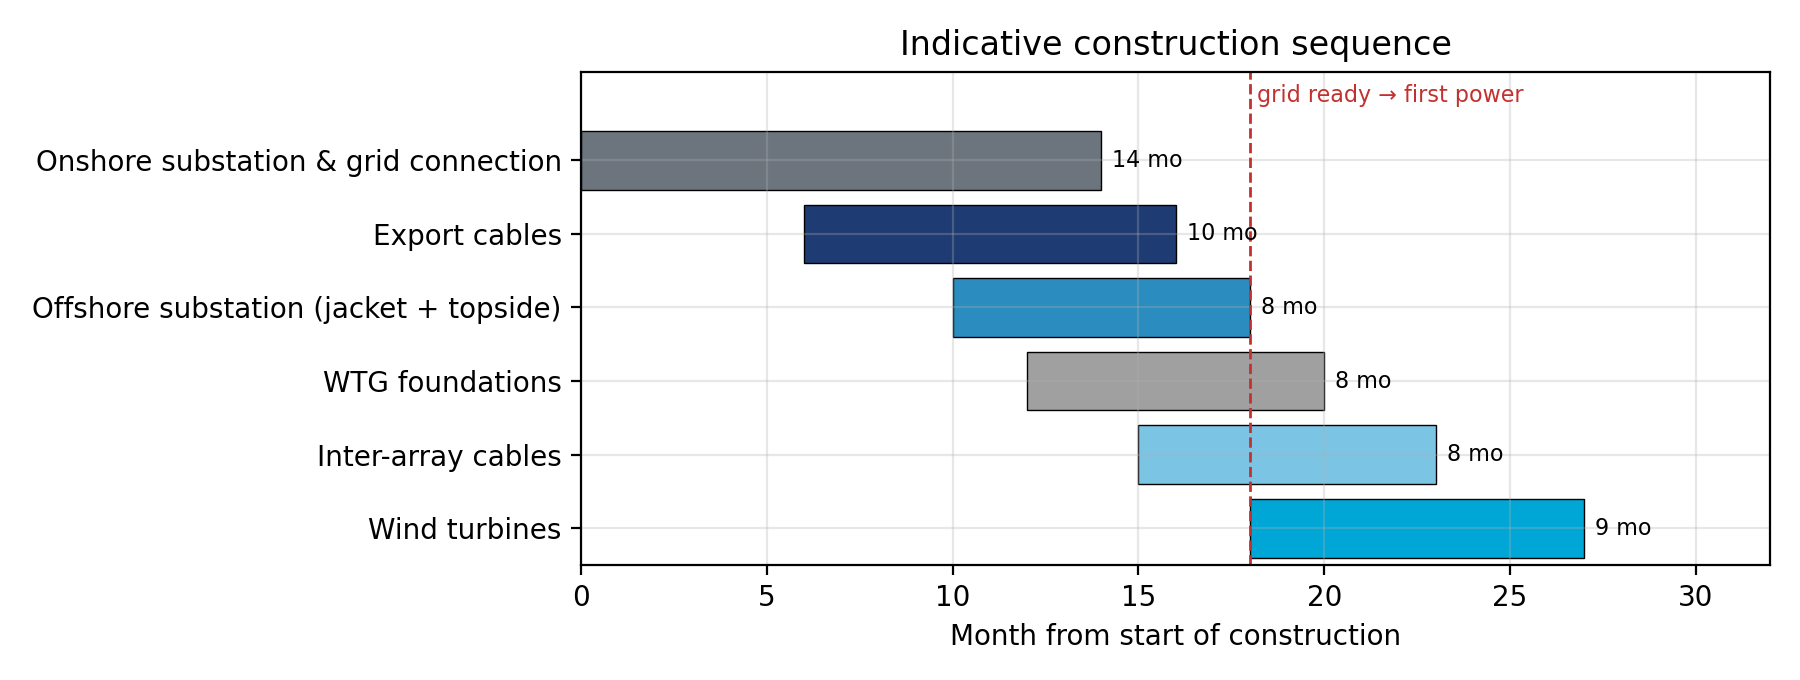
\includegraphics[width=0.8\textwidth]
    {figures/electrical/p4_construction_gantt.png}
    \caption{Indicative construction sequence: the grid connection and export system are ready when WTG installation starts.}
    \label{fig:elec-gantt}
\end{figure}

\begin{figure}[H]
    \centering
    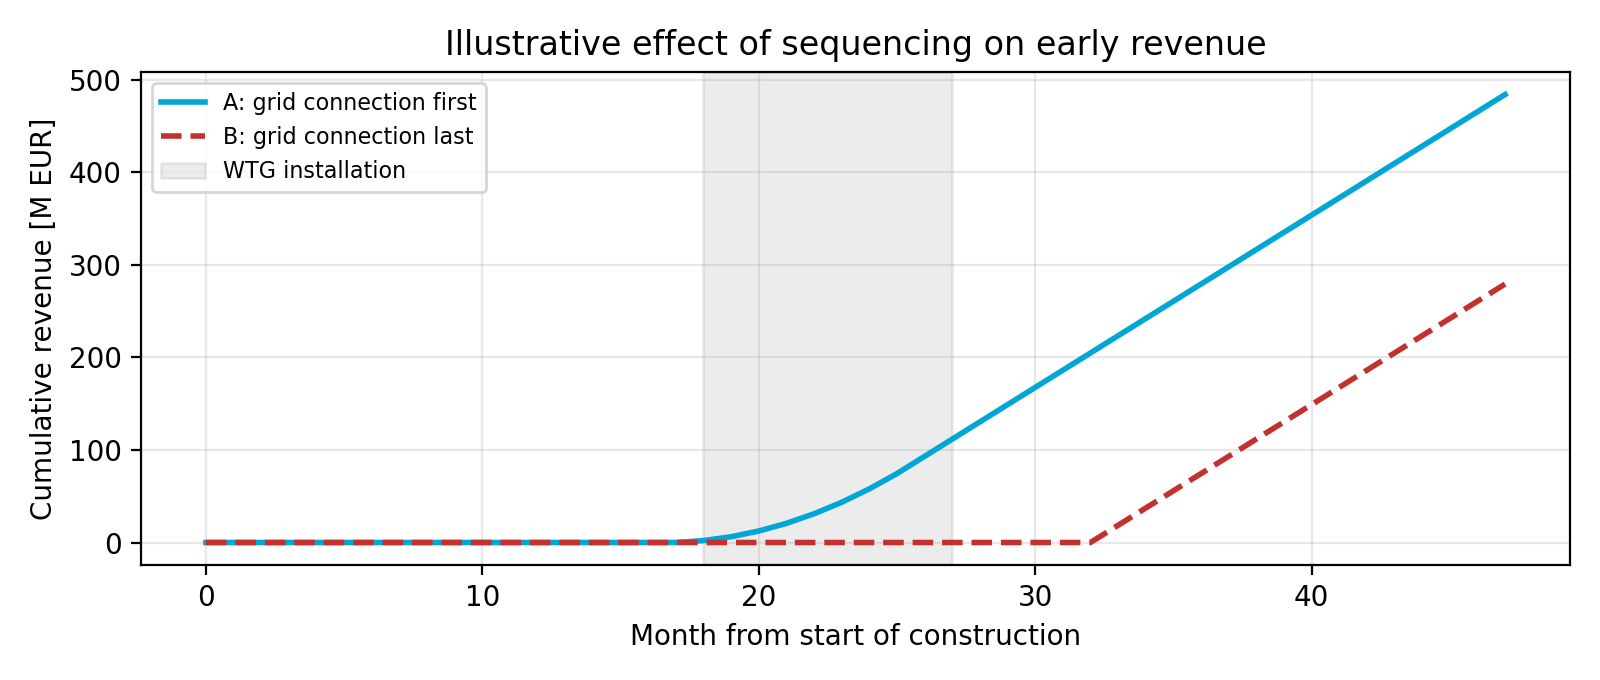
\includegraphics[width=0.7\textwidth]
    {figures/electrical/p4_revenue_sequence.png}
    \caption{Illustrative cumulative revenue for grid-first versus grid-last sequencing, using the same WTG installation campaign.}
    \label{fig:elec-revenue}
\end{figure}

\section{Feedback}
\label{sec:elec-feedback}
\begin{quote}
\emph{Offshore Renewable Technology is a new course. As your lecturers, we are motivated to learn with you and improve going forward. Therefore, we very much appreciate feedback on our work. Please provide your constructive feedback to the ORT-course thus far -- it can be on lectures, course material, assignments and you are also welcome to make suggestions. [1 pts]}
\end{quote}

% TODO (Group 21): adapt this draft to your own experience before submitting.
The lectures on electrical design connected theory and practice well. Real project examples, such as the Windpark Fryslân timeline from concept design to final design, made clear why choices about voltage level, number of export cables and redundancy are made. The Excel templates made the assignments concrete and easy to check step by step.

We have three suggestions. First, a short worked example of one row of the `IAC' tab during the lecture would make the expected method clearer, for example the role of $\cos\varphi$ and of the hours per bin. Second, some template cells contain fixed or rounded values, such as the hours of the first and last bin and the $21.1\,\mathrm{MVA}$ rating; a short note in the template would avoid confusion. Third, publishing all slides before the lecture, together with a list of the key formulas (three-phase power, losses, redundancy), would help us prepare for both the lectures and the exam.


\end{document}
